% =============================================================================
% paper_wp.tex: working-paper version. Same text as the AEJ: Economic Policy
% submission (sections/body.tex), with the authors, a single-column layout
% for reading on screen, live links, and the Online Appendix
% (sections/appendix_body.tex) appended after the references.
% =============================================================================
\documentclass[12pt]{article}
\usepackage[T1]{fontenc}
\usepackage{lmodern}
\usepackage[letterpaper, margin=1in]{geometry}
\usepackage{amsmath}
\usepackage{booktabs}
\usepackage{graphicx}
\usepackage{natbib}
\usepackage{url}
\urlstyle{same}                    % the bibliography sets URLs in italics, where typewriter type spaces out every dot
\usepackage{setspace}
\setstretch{1.3}
\frenchspacing                      % one interword space after a full stop
\usepackage{etoolbox}
\AtBeginEnvironment{table}{\renewcommand{\arraystretch}{0.88}}   % tighter rows, so the tallest table fits the 12pt page
\usepackage[labelfont=bf, labelsep=period, font=small]{caption}
\captionsetup[table]{position=above, skip=6pt}
\usepackage[hidelinks]{hyperref}
\usepackage[dvipsnames]{xcolor}
\hypersetup{colorlinks=true, linkcolor=MidnightBlue, citecolor=MidnightBlue, urlcolor=MidnightBlue}

% The notes environments of the AEA template, so the shared text compiles here.
\newenvironment{tablenotes}[1][Note]{\par\vspace{5pt}\noindent\begin{minipage}{\linewidth}\footnotesize\setstretch{1}\textit{#1:} }{\end{minipage}\par}
\newenvironment{figurenotes}[1][Note]{\par\vspace{5pt}\noindent\begin{minipage}{\linewidth}\footnotesize\setstretch{1}\textit{#1:} }{\end{minipage}\par}

\renewcommand{\topfraction}{0.9}
\renewcommand{\bottomfraction}{0.6}
\renewcommand{\textfraction}{0.07}
\renewcommand{\floatpagefraction}{0.75}
\graphicspath{{../analysis/output/graphs/}}
\newcommand{\tabdir}{../analysis/output/tables}

\title{\textbf{Darker Evenings: Road Deaths after Brazil Abolished Daylight Saving Time}}
\author{Fredie Didier\thanks{\raggedright Instituto Brasileiro de Ensino, Desenvolvimento e Pesquisa (IDP), Bras\'ilia, DF, Brazil. Email: fdidier@terra.com.br.} \and Leonardo Monasterio\thanks{\raggedright Instituto de Pesquisa Econ\^omica Aplicada (Ipea), Rio de Janeiro, RJ, Brazil, and Instituto Brasileiro de Ensino, Desenvolvimento e Pesquisa (IDP), Bras\'ilia, DF, Brazil. Email: leonardo.monasterio@idp.edu.br.}}
\date{Working paper, \today}

\begin{document}
\begin{titlepage}
\maketitle
\begin{abstract}
\noindent% Abstract: at most 100 words (AEJ: Economic Policy). Count with
%   grep -v '^%' sections/abstract.tex | wc -w
In 2019 Brazil abolished daylight saving time, moving an hour of summer light from evening to morning for 131 million people. I compare road deaths in the clock hour that turned dark, located for each municipality and day, with the same hour before abolition and in states that never had it. Deaths in that hour rose 34 percent; pedestrians, 12 percent of these deaths before, account for 43 percent of the increase. The morning hour that gained light shows no offsetting decline. Abolition cost 54 lives per summer, a lower bound. Mexico's 2022 abolition shows the same pattern.


\medskip\noindent\textbf{JEL:} I18, R41, O54\\
\textbf{Keywords:} daylight saving time, ambient light, road deaths, pedestrians, Brazil
\end{abstract}
\thispagestyle{empty}
\end{titlepage}

% =============================================================================
% body.tex: the text of the paper, from the introduction to the conclusion,
% with the main-text exhibits. Read by paper.tex (submission) and
% paper_wp.tex (working paper). Every number comes from the tables and figures
% generated by analysis/code/27_figures.R and 28_tables.R, or from the caches
% in audit/*.rds that those scripts read; the source of each number that no
% exhibit prints is given in a comment beside it.
% =============================================================================

\introsection

In modern societies clocks set the hours at which people work and sleep \citep{hamermesh2008cues}. Daylight saving time (DST) moves the clock forward by an hour in summer, which shifts an hour of daylight from the morning to the evening. Whether to keep changing the clocks every year is an open question in many countries. Mexico abolished DST in 2022, the European Parliament voted in 2019 to end seasonal clock changes, and the US Senate in 2022 and the House of Representatives in 2026 each passed a bill that would make DST permanent \citep{mexico2022ley, europarl2019seasonal, uscongress2022sunshine, uscongress2026sunshine}. Brazil, which had moved its clocks every summer since 1985, abolished DST in April 2019 \citep{brasil2019decreto}, after its Ministry of Mines and Energy concluded that DST no longer saved electricity \citep{mme2019nota}. By then DST applied only in the South, Southeast, and Center-West, the 11 states where 131 million of Brazil's 203 million people (65 percent) lived, according to the 2022 Census \citep{ibge2023censo}. In those states the sun has since set an hour earlier on the clock from November to February. While the debate, in Brazil and elsewhere, has largely focused on electricity \citep{kellogg2008daylight, kotchen2011does}, clock time also determines whether the evening commute occurs in daylight or after dark. The stakes on the road are large: crashes killed 37,150 people in Brazil in 2024, 15 percent of them pedestrians \citep{datasus2025sim}. % national_road_deaths.rds (13_design_descriptives.R): 2024, 37,150 deaths, 15.3 percent pedestrians.

The clock rule a country chooses can affect road deaths because daily activities are coordinated: work and leisure are worth more when they coincide with other people's schedules \citep{hamermesh2008cues}. A clock rule therefore shifts society's entire day relative to daylight at once. Three forces then set its cost on the road. First, people respond to known hazards by reducing their exposure, so observed harm reflects these avoidance responses \citep{neidell2009information}. On the road, avoidance may involve shifting travel away from hours that have become dark. Second, schedules respond to the clock: under DST, people appear to move some activities earlier in the day \citep{sexton2014behavioral}. Third, drivers do not fully internalize the risks their driving imposes on others \citep{edlin2006accident}, including pedestrians and cyclists \citep{crandall1984automobile, white2004arms}. These mechanisms do not establish the net effect on road deaths after travel patterns adjust, including whether brighter mornings offset the additional deaths caused by darker evenings. The evidence on DST and road safety comes mostly from the clock changes themselves, comparing crashes in the days or weeks just before the clocks move with those just after \citep{sullivan2002role, sood2007short, smith2016spring, laliotis2023summertime, gillmore2025daylight}. A clock change shifts daylight relative to clock time overnight. Because work and school schedules remain largely unchanged, comparisons around the transition capture the effect of the change in light before travel patterns have had time to adjust. Each change also adds a second shock, a night with an hour more or less of sleep. Studying a change in the time regime over several seasons avoids both limitations: there is no one-night sleep shock, and travel patterns have time to adjust.

This paper uses Brazil's abolition of DST to estimate how many additional road deaths occur once travel patterns have adjusted to darker evenings, and whether brighter mornings offset those deaths. Abolition turned one hour of every summer evening from daylight to darkness. In S\~ao Paulo in mid-January, for example, the sun set at 7:58 p.m.\ on the clock under DST and now sets at 6:58 p.m., so the hour from 6:58 to 7:58 p.m.\ was the last hour of sunlight under DST and has been the first hour after sunset since abolition. We call it the hour that turned dark. It is the hour after sunset in standard time, the clock without DST, so it falls at a different clock time in each municipality and on each date. We compute that hour from the solar position at each municipal seat on each date, and do the same for the hour after standard-time sunrise, which went the other way, from darkness to daylight. We use a triple-difference design that compares the 11 states observing DST in every southern-hemisphere summer from 2008/09 to 2018/19 with 12 states that did not. The estimate contrasts changes before and after abolition in the gap between the summer window and April--August, focusing on the hour that turned dark. Because the affected hour follows local sunset across municipalities and dates, a confounding regional trend would need to align with this shifting hour to explain the estimate. The hours immediately before and after experienced smaller changes in light and therefore provide a further check on whether the response follows the change in light. A second design uses every clock hour of the day, each weighted by how much darker or lighter abolition made it. With a separate effect for each clock hour on each date, it tests whether the deaths follow the sun or the clock, and it counts the net change over the day without selecting particular hours.

Two independent high-quality sources measure the outcome. The Ministry of Health's Mortality Information System (SIM) provides death certificates covering fatalities on all public roads in the country. For deaths at the crash scene, the recorded time of death closely approximates the time of the crash. The publicly available crash records of the Federal Highway Police (PRF) cover every crash its officers respond to on federal highways, together with the light conditions the officers recorded at the crash scene. These records confirm the change in light: in the hour that turned dark, the share of crashes that officers recorded as occurring at dusk or at night rose by 24 percentage points after abolition.

We estimate that, after abolition, road deaths in the hour that turned dark rose by 29.2 log points (34 percent), from an average of 110 per summer in the 11 treated states. Deaths and injury crashes on federal highways rose by 54 and 22 log points (71 and 25 percent). Each estimate remains significant under three forms of inference that do not rely on asymptotics with 23 clusters: a score wild bootstrap of the Poisson model, a wild cluster bootstrap of its linear analogue, and a permutation of the treated states. The effect follows the local sun rather than the clock. With clock-hour-by-date fixed effects, we estimate a 48-log-point increase in road deaths when an evening hour shifts from full daylight to night. The estimate remains similar when identification relies only on differences in sunset times across treated states and summer dates.

For road deaths, the season-by-season estimates before abolition show no differential trend. Without the pandemic months the estimate is 23 log points; in the summer window alone, without the off-season comparison, it is 34 and stable across the five seasons without DST. An imputation estimator that extrapolates the pre-abolition trend yields a similar point estimate, although with substantially less precision. On federal highways, injury crashes show a trend before abolition, and both federal highway estimates shrink once a trend is allowed. We therefore take the magnitude of the effect from road deaths and use federal highway records to verify the change in light and to investigate the mechanisms. The rise is concentrated in the hour that turned dark and the next one, which went from twilight to night. Road deaths at midday and at night, whose light did not change and where an effect of sleep would also appear, do not rise.

Pedestrians bear a disproportionate share of the increase in deaths. They were 12 percent of road deaths in the hour that turned dark before abolition and account for 43 percent of the excess after it. Their deaths in that hour more than doubled, a rise of 77 log points (115 percent), compared with 18 log points (20 percent) for all other road users. The estimate for all road deaths is also larger in municipalities where more households live on block faces without street lighting (42.5 log points, compared with 10.9 where streets are better lit), although the difference is imprecise ($p=0.10$). Travel responded to light as well. Hourly counts at the federal highway stations of the National Traffic Count Plan show that traffic in the hour that turned dark fell by about 6 percent and traffic in the morning hour that turned light rose by about 12 percent. Under permutation inference, the first change is borderline and the second is not significant. Over the summers covered by the traffic counts, the risk of an injury crash per vehicle in the hour that turned dark rose by 24 log points (27 percent), more than crashes themselves.

Road deaths in the hour after sunrise, which turned light, show no detectable change ($-3$ log points, standard error 12). For the same change in darkness, the estimated effect on road deaths is larger in the evening than in the morning (permutation $p=0.001$). In the hour that turned dark, road deaths exceeded the counterfactual by 36 per summer window, an estimate that requires no assumption about the other hours of the day. A count for the whole day requires an assumption about those hours. When every hour of the day is weighted by how much darker or lighter it became, and hours that remained in full daylight or full darkness are assumed unaffected, abolition added 62 road deaths per summer window, from November 15 to February 14 (standard error 12; permutation $p=0.001$). The count includes only deaths at the crash scene with a recorded time. Estimated over the whole day without assuming that hours whose light did not change were unaffected, the change is too imprecise to confirm the count or rule it out. A decline in deaths in the hours whose light did not change, large enough to cancel the count, could come from trips moving out of those hours, but the traffic counts show no such shift. They cannot exclude a smaller decline.

At a value of a statistical life adjusted to Brazil's income level \citep{robinson2019valuing}, the 62 additional deaths in each summer window add up to an estimated cost of 114 million 2025 international dollars, rising to 287 million when the count is scaled up to include deaths with no recorded time and deaths that occurred off the road, mostly in hospitals. Over a whole DST season the cost is 135 million.

The clock changes before 2019 show the same change of light before travel had time to adjust: for three weeks after each change, the evening hour was dark (after February) or light (after October) while travel kept to the same clock hours. Read as the effect of a darker evening, the changes give 42 log points (standard error 14) and abolition 29. The 29 log points are an average over the whole summer window, however. Abolition raised road deaths in the hour that turned dark by 58 log points (13) from mid-November to early December and by 49 (16) in the second half of January, but left no detectable change from Christmas to mid-January. The weeks after the clock changes fall while schools are in session, as do the weeks from mid-November to early December. In those weeks the effect of abolition is statistically indistinguishable from the effect at the clock changes, whether the hour that turned dark is compared across states or with other hours of the same day. We find no sign that, five summers after abolition, the effect of a darker evening had faded as travel adjusted, although the comparison cannot rule out a moderate decline.

The paper relates to three literatures. The first estimates the effect of DST on road safety, mostly from the clock changes: in the United States \citep{sood2007short, smith2016spring}, Australia \citep{james2023let}, Greece \citep{laliotis2023summertime}, Chile \citep{gillmore2025daylight}, and Mexico \citep{goodwin2024impact}. These studies attribute the deaths that follow the spring change to lost sleep \citep{smith2016spring, gillmore2025daylight}, and find that the light DST adds to the evening lowers serious crashes \citep{laliotis2023summertime, gillmore2025daylight} or mainly moves deaths between hours of the day \citep{smith2016spring}. For Brazil, \citet{franco2023daylight} use federal highway records from 2007 to 2012 and find that total crashes fall when DST starts, with more crashes near sunrise and fewer near sunset, and that the effect of light persists while DST is in force. We study the end of DST instead of its start, count deaths on all public roads, and observe the five summers after the clock changes stopped. \citet{depalo2023should}, who explicitly asks whether DST should be abolished, also relies on clock transitions to answer that question. Closest to the question of regimes, \citet{bunnings2021spring} estimate the effect of darkness on crashes in Great Britain from the variation in sunrise and sunset times across places and dates, and simulate that year-round DST would save 8 percent of the cost of darkness. \citet{coate2004effects} estimate that year-round DST would avoid 171 pedestrian deaths a year in the United States, and \citet{ferguson1995daylight} that it would have avoided about 900 fatal crashes in 1987--1991, four fifths of them involving pedestrians. \citet{james2023let} also uses the trials of DST in Australian states and its extension for the Sydney Olympics, and finds no long-run effect on road deaths, only a reallocation of crashes across the hours of the day.

The second literature uses DST to identify the effect of ambient light on behavior, mostly crime \citep{doleac2015under, tealde2022unequal, dominguez2023crime}; in Brazil, homicides by firearm fell during the months of DST, mostly in the early-evening hours that DST lit \citep{toro2016daylight}. These studies look for the effect in the hours whose light the clock moves. Here the shift of light is permanent, and it arrives without the change in sleep that a clock change brings. Russia's reforms of time-zone boundaries over four decades also shifted light persistently: the daylight regime had a lasting effect on women's sense of safety and an immediate one on the time people spent walking for transport \citep{jelnov2027sunset}.

The third literature weighs the costs and benefits of DST. It has mostly measured energy use \citep{kellogg2008daylight, kotchen2011does} and, through sleep, health and productivity \citep{gibson2018time, giuntella2019sunset, jin2020sleep, osbornechristenson2022saving, jagnani2024children}. The road-safety studies above mostly measure the transitions, which a choice between permanent regimes removes either way.

Relative to these literatures, the paper makes the following contributions. First, it estimates the road-safety consequences of an actual change in clock regime, observed over five summers, rather than inferring them from short windows around clock transitions or from simulations, and it compares them with the same change of light at the clock changes, before travel adjusted. Second, because the hour that turned dark is set by the local sun, the design separates the effect of darkness from the effects of the clock and of sleep, and it shows that the evening hour that lost light became deadlier, disproportionately for pedestrians, while the morning hour that gained light did not become detectably safer.

% -----------------------------------------------------------------------------
\section{Daylight Saving Time in Brazil and Its Abolition}\label{sec:background}

\subsection{The policy}

Brazil observed DST every summer from 1985/86 to 2018/19. Which states observed it changed often in the 1990s. From 2008, a standing decree fixed both the dates and the states \citep{brasil2008decreto}. Clocks moved forward at midnight on the third Sunday of October (from 2018, the first Sunday of November; \citealp{brasil2017decreto}) and back on the third Sunday of February (a week later when that Sunday was Carnival Sunday). DST applied in Rio Grande do Sul, Santa Catarina, Paran\'a, S\~ao Paulo, Rio de Janeiro, Esp\'irito Santo, Minas Gerais, Goi\'as, Mato Grosso, Mato Grosso do Sul, and the Federal District, which held 131 million of Brazil's 203 million people in 2022 \citep{ibge2023censo}. Within the sample, Bahia had DST only in 2011/12 and Tocantins only in 2012/13 \citep{brasil2011decreto, brasil2012decreto, brasil2013decreto}. The North and the rest of the Northeast, close to the equator, where the length of the day varies little over the year, did not have DST in this period. Figure~\ref{fig:map} maps the groups.

Presidential Decree 9,772 of April 25, 2019, abolished DST in the whole country \citep{brasil2019decreto}. It followed a technical note of the Ministry of Mines and Energy that concluded that DST had stopped delivering the electricity savings it was designed for \citep{mme2019nota}. In 2024 a technical note of the national grid operator reached the opposite conclusion: it finds that DST would benefit the power system, because the growth of distributed generation has moved the peak in the demand it supplies to the evening \citep{ons2024nota}.

\begin{figure}[tbp]
  \centering
  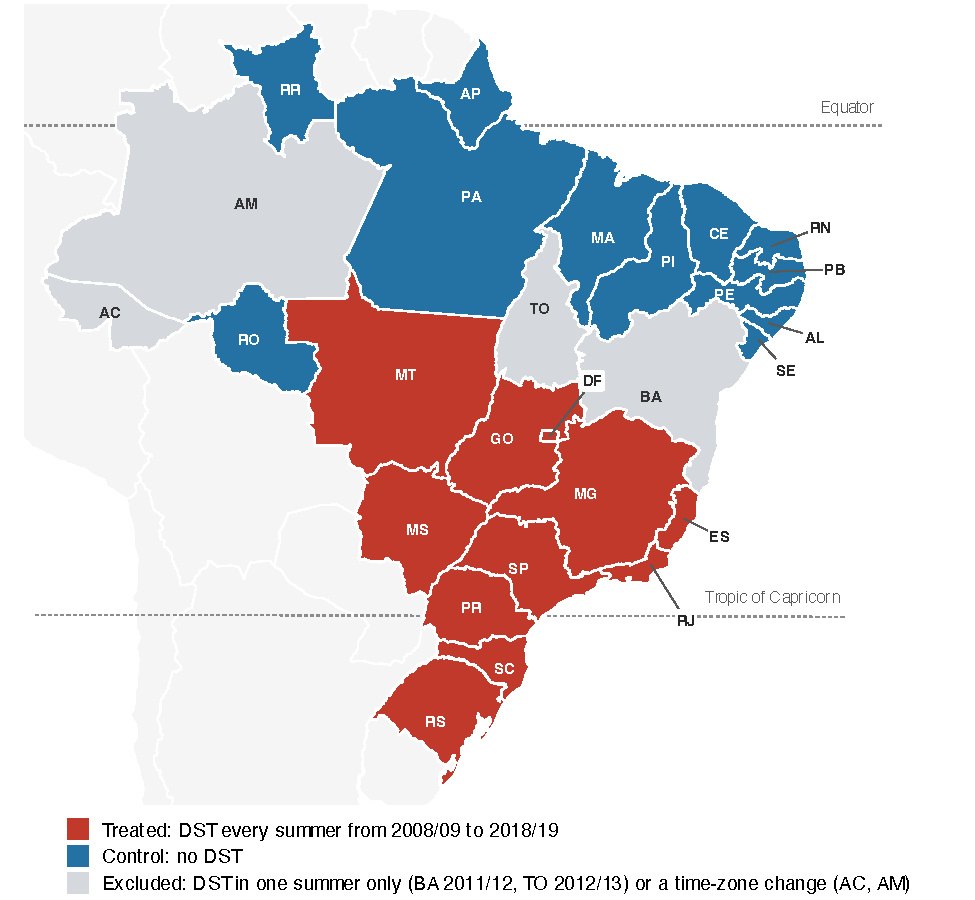
\includegraphics{../analysis/output/maps/fig_map_brazil.pdf}
  \caption{Treated and Control States}
  \label{fig:map}
  \begin{figurenotes}[Notes]
  Treated states had DST every summer from 2008/09 to 2018/19 and none afterward. Control states had no DST in any summer of the sample. Bahia (2011/12) and Tocantins (2012/13) had DST in a single summer of the sample; Acre and the west of Amazonas moved their clocks to another time zone in 2008 and back in 2013. The west of Par\'a, a control state, changed time zone in June 2008, before the sample begins.
  \end{figurenotes}
  \begin{figurenotes}[Sources]
  Decrees 6,558/2008, 7,584/2011, 7,826/2012, 8,112/2013, 9,242/2017, and 9,772/2019; state boundaries, \citet{ibge2020malha}; other countries, \citet{naturalearth}.
  \end{figurenotes}
\end{figure}

\subsection{What abolition changed}

Panel A of Figure~\ref{fig:light} shows the clock time of sunset and sunrise in S\~ao Paulo over 2018/19, under the DST then in force and without it. In mid-January the sun set at 7:58 p.m.\ on the clock under DST and now sets at 6:58 p.m.; it rose at 6:32 a.m.\ and now rises at 5:32 a.m. % São Paulo, January 15, NOAA equations (EXPLICANDO_O_PROJETO.md, section 1.2).
Because work, school, and the commute keep to the clock, abolition put the people who used to travel in the last hour of sunlight on the road after sunset.

\begin{figure}[tbp]
  \centering
  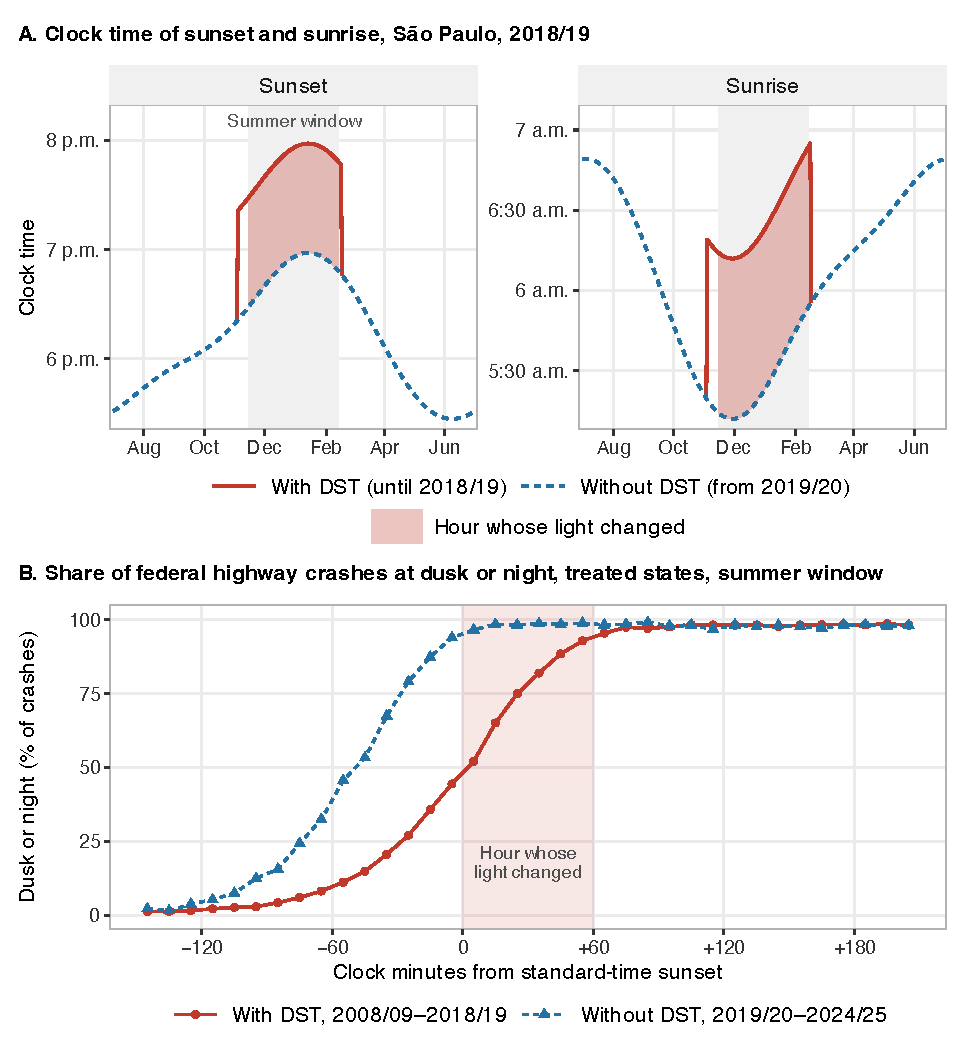
\includegraphics{fig_light.pdf}
  \caption{The Hour Whose Light Changed}
  \label{fig:light}
  \begin{figurenotes}[Notes]
  Panel A: S\~ao Paulo, July 2018 to June 2019. The solid line is clock time under the DST in force that season (November 4, 2018, to February 17, 2019); the dashed line is clock time without DST, the rule since 2019/20. The grey band is the summer window used in every season. The shaded hour after standard-time sunset was light with DST and is dark without it; the hour after standard-time sunrise is the reverse. Panel B: federal highway crashes in the 11 treated states, summer window; share of crashes recorded as occurring at dusk or at night, by 10-minute bin of clock time minus standard-time sunset at the municipality of the crash. The shaded hour is hour 0.
  \end{figurenotes}
  \begin{figurenotes}[Source]
  Panel B: \citet{prf2025dados}.
  \end{figurenotes}
\end{figure}

Let $s_{md}$ be the clock time of sunset in standard time at municipality $m$ on day $d$. Under DST the clock ran an hour ahead, so the sun set at clock time $s_{md}+60$ minutes and was above the horizon throughout the clock hour $[s_{md}, s_{md}+60)$. Since abolition the sun has been below the horizon throughout that hour. We call it hour 0, or the hour that turned dark. Its morning counterpart, the clock hour $[r_{md}, r_{md}+60)$ after standard-time sunrise $r_{md}$, was dark under DST and is light now. The neighboring hours changed less: the hour before $s_{md}$ went from full sun to low sun, and the hour after $s_{md}+60$ from twilight to night.

% -----------------------------------------------------------------------------
\section{Data}\label{sec:data}

\paragraph{Deaths on the road}

The Mortality Information System (Sistema de Informa\c{c}\~oes sobre Mortalidade, SIM) of the Ministry of Health holds every death certificate issued in Brazil, with the underlying cause of death coded in the International Statistical Classification of Diseases and Related Health Problems, 10th Revision (ICD-10), the municipality and type of place of occurrence, and the date and clock time of death \citep{datasus2025sim}. We select deaths from land-transport crashes (codes V01--V89) that occurred on a public road and call them road deaths. For a person who dies at the crash scene, the time of death is close to the time of the accident: when a federal highway crash with one death and a single road-death certificate fall in the same municipality and day, the certificate's time lies within the hour after the crash in 59 percent of the pairs, compared with 5 percent for pairs formed a week apart (Online Appendix Table~\ref{tab:measurement}). For a person who dies in a hospital, it may be hours or days later. In-hospital deaths therefore never enter an hourly count. Between 15 and 20 percent of road-death certificates, depending on the group of states, the time of year, and the period, provide no clock time, and those deaths drop out of every count as well. % pretrends.rds, missing_hour: 15.4 to 20.1 percent by group, window and period.
Abolition had no detectable effect on the share of road deaths without a clock time: the triple-difference estimate is 0.4 percentage points (standard error 0.7; Online Appendix Figure~\ref{fig:records} and Table~\ref{tab:measurement}). % record_integrity.rds, test: no_time 0.425 (0.652).
However, the composition of the deaths without a clock time changed. After abolition, pedestrians' share of these deaths rose by 2.9 percentage points (standard error 1.2), while their share of deaths with a clock time did not change ($-0.3$, standard error 0.8). If more pedestrian deaths lost their clock time after abolition, our hourly counts would miss those deaths, so our pedestrian estimates would be too low, not too high. % record_integrity.rds, test: ped_no_time 2.858 (1.233), p = 0.030; ped_time -0.286 (0.770).
In the treated states, an average summer window before abolition had 2,382 road deaths with a clock time, 110 of them in hour 0 (Table~\ref{tab:descriptives}).

The death registry is the standard source on mortality in Brazil, including in economics \citep[for example,][]{dixcarneiro2018economic}. Its coverage rests on a legal requirement: no burial may take place without a death record, which the registry office issues on the basis of a physician's death certificate where a physician is available \citep[art.~77]{brasil1973lei}. DST abolition did not change how deaths are recorded. In a triple difference, the share of land-transport deaths that occur on the road (half of them) does not move with abolition either (Online Appendix Figure~\ref{fig:records} and Table~\ref{tab:measurement}).

\paragraph{Crashes on federal highways}

The Federal Highway Police (Pol\'icia Rodovi\'aria Federal, PRF) publishes every crash its officers respond to on federal highways, from 2007 to 2025, with date, clock time, municipality, numbers of people killed and injured, type of crash, and the light conditions as recorded by the officer: full daylight, dawn, dusk, or night \citep{prf2025dados}. We use two outcomes. Federal highway deaths count people killed at the crash scene \citep{prf2025anuario}, the same concept as road deaths in the SIM. Federal highway injury crashes are crashes with at least one casualty, a person killed or injured. We do not use crashes without casualties. For these crashes, an online report filed by those involved gradually replaced on-scene police response, and this happened at different dates in different states, so their recorded number is not comparable over time between the treated and control states. The two sources only partially overlap. Road deaths cover every public road, urban streets included; federal highways run mostly outside urban areas, where the treated states had 1,176 deaths per summer before abolition, compared with 2,382 road deaths (Table~\ref{tab:descriptives}).

\paragraph{Traffic flow}

The National Traffic Count Plan (Plano Nacional de Contagem de Tr\'afego, PNCT) of the federal roads agency (DNIT) publishes hourly vehicle counts, by direction and vehicle class, at continuous counting stations on federal highways \citep{dnit2025pnct}. We use complete station-days counted from 2014 to May 2019 and from May 2021 to 2025, which cover the summers 2014/15 to 2018/19 and 2021/22 to 2024/25.\footnote{DNIT's contract for continuous counts ended in June 2019. The values published for the second half of 2019 were estimated with a statistical model, and there were no counts in 2020 \citep[p.~7]{dnit2020nota}. A new contract was tendered in 2020 \citep{dnit2020edital} and signed on December 30, 2020, and January 13, 2021; counting resumed in May 2021. We drop every station-day from June 2019 to December 2020, and any station-day whose daily total repeats exactly on the same weekday one to four weeks apart, which marks a modeled value.}

\paragraph{Sun and clock}

For each municipal seat and day we compute sunrise and sunset in standard time from the solar position equations of \citet{noaa2025solar}, using the seat coordinates from IBGE \citep{ibge2010sedes, ibge2020municipios} and the standard offset of the municipality's legal time zone \citep{brasil1913decreto, brasil2008lei, brasil2013lei}. Every death and crash is then placed in a 60-minute bin of clock time relative to standard-time sunset or sunrise at its municipality on its date. Using NOAA's full solar algorithm \citep{meeus1998astronomical} instead moves sunset by at most 1.6 minutes and the main estimate from 29.2 to 29.8 log points (Online Appendix Table~\ref{tab:measurement}). The death certificates, the federal highway police records, and the traffic counts all give legal clock time, the time on the clock under whatever regime was in force. Section~\ref{sec:firststage} shows this in the officers' records, and Online Appendix~\ref{app:data} in the death certificates and the traffic counts.

\paragraph{Sample}

The treated group consists of the 10 states that had DST every summer from 2008/09 to 2018/19 and the Federal District, which contains the capital, Bras\'ilia, and has the powers of a state. We refer to these 11 units as the treated states. The control group is the 12 states of the North and Northeast without DST in the sample: Rond\^onia, Roraima, Par\'a, Amap\'a, Maranh\~ao, Piau\'i, Cear\'a, Rio Grande do Norte, Para\'iba, Pernambuco, Alagoas, and Sergipe. We exclude Bahia and Tocantins, which had DST in one summer each, and Acre and Amazonas, which changed time zone during the sample (Figure~\ref{fig:map}). Online Appendix Figure~\ref{fig:bahia} uses Bahia's single summer with DST, 2011/12, as a check of sign. A season runs from July to June, so that each summer falls within one season, and is named by its first year. The sample runs from 2008/09, the first season under the 2008 decree, to 2023/24, the last for which the death registry is final, so it has 11 seasons with DST and 5 without.

The summer window runs from November 15 to February 14. Every day in it was under DST in every season before abolition: the latest start of DST in the sample was November 4, 2018, and the earliest end February 15, 2009. The same window is used in every season, before and after abolition, so no day in it is partly treated and the year-to-year variation in DST dates does not enter the comparison. The window starts at least 11 days after the latest start of DST and ends before the earliest end, so the weeks after clock changes, when the literature finds the effects of lost sleep \citep{smith2016spring, gillmore2025daylight}, fall outside it. The off-season runs from April 1 to August 31, when no state ever had DST. The estimation panel has one row per state and day in these two windows: 23 states and 245 days in each of 16 seasons, or 90,160 state-days.

\begin{table}[tbp]
  \caption{Events per Summer by Group, Window, and Period}
  \label{tab:descriptives}
  \centering\footnotesize\setlength{\tabcolsep}{3.5pt}
  \input{\tabdir/tab_descriptives.tex}
  \begin{tablenotes}[Notes]
  Average count per season. Before: 2008/09 to 2018/19 (11 seasons); after: 2019/20 to 2023/24 (5 seasons). Summer window: November 15 to February 14; off-season: April 1 to August 31. Only events with a recorded clock time.
  \end{tablenotes}
  \begin{tablenotes}[Sources]
  \citet{datasus2025sim}; \citet{prf2025dados}.
  \end{tablenotes}
\end{table}

Table~\ref{tab:descriptives} shows the counts the design compares. In the treated states, road deaths in hour 0 rose from 110 to 141 per summer after abolition, while those in the same hour of the off-season fell from 362 to 313; in the control states both fell. Taken together as a triple difference in logs, these changes amount to about 29 log points (33 percent). Pedestrian deaths in hour 0 of the treated states' summer doubled, from 13 to 27 per summer, while they fell in the off-season and in the control states.

% -----------------------------------------------------------------------------
\section{Empirical Strategy}\label{sec:design}

\subsection{Specification}

For each state $s$ and day $d$ in the summer window or the off-season, let $y_{sd}$ count the events that occur in one hour bin, hour 0 unless stated otherwise. The main specification is
\begin{equation}\label{eq:main}
  y_{sd} = \exp\big(\beta\, T_s W_d A_d + \alpha_{s,w(d)} + \gamma_{s,t(d)} + \delta_d\big)\,\varepsilon_{sd},
\end{equation}
where $T_s$ marks the 11 treated states, $W_d$ days in the summer window, and $A_d$ seasons after abolition. The fixed effects are state by window ($\alpha$; summer window or off-season), state by season ($\gamma$) and date ($\delta$). We report $100\beta$, the effect in log points.

Each set of fixed effects removes a class of threats. State-by-window effects absorb every permanent difference between a state's summer and its off-season: tourism, the rainy season, and the fact that hour 0 falls at a later clock time in summer than in winter. State-by-season effects control for anything that moves a state's counts proportionally in both windows of a season, such as its vehicle fleet, enforcement, or the pandemic. Date effects absorb national holidays and national shocks. The coefficient $\beta$ is then identified by the change, after abolition, in the gap between the summer and the off-season of the treated states, relative to the same change in the control states. The identifying assumption is that the gap would have moved in parallel in the two groups had DST not been abolished.

We estimate Equation~(\ref{eq:main}) by Poisson pseudo-maximum likelihood, which requires only that the conditional mean be correct and handles the many zeros of a single hour's count \citep{santossilva2006log}: 88 percent of state-days have no road death in hour 0. The share of zeros implied by the fitted means matches the observed share within 1.1 percentage points in every outcome, and the ratio of the residual variance to the mean is between 0.9 and 1.6, so neither a zero-inflated nor a negative binomial model is needed. % inference.rds: zeros_obs_pct against zeros_poisson_pct, largest gap 1.05 (federal highway deaths, morning); dispersion 0.93 to 1.57.

We use a single hour as the outcome because, within the summer window alone, standard-time sunset differs across the municipalities of the sample by about two hours, so a fixed block of clock hours mixes hour 0 with hours whose light did not change and dilutes the effect. The definition of hour 0 also implies where an effect of darkness must appear and where it must not. A shock to the treated states' summers unrelated to darkness, such as a change in policing, has no reason to concentrate in the hour that follows standard-time sunset at each municipality on each date and to leave the hours on either side of it unaffected.

\subsection{Darkness or the clock: the dose model}\label{sec:dose}

Interpreting the hour-0 estimate as the effect of darkness requires that no other post-2019 change systematically affected the clock times at which hour 0 occurs. In the treated states' summer it falls later on the clock than in their off-season (in S\~ao Paulo, about 7 p.m.\ in January and 5:30 p.m.\ in June) and later than in the control states, closer to the equator. A change after 2019 in the risk at that time of the evening, anywhere in the country, would therefore bias $\beta$. A second design separates darkness from clock time. For each municipal seat, date, and clock hour $h$, we compute from the solar position how dark the hour is without DST and how dark it was with it, counting a minute of night as 1, a minute of civil twilight (the sun less than six degrees below the horizon) as one half, and a minute of daylight as 0. The difference is the change in darkness abolition brought to that clock hour. It runs from 1, for an evening hour that went from full daylight to night, to $-1$, for a morning hour that went the other way, and it sums to zero over each day. Averaged over each state's municipal seats, weighted by their road deaths before abolition, it gives $D_{sdh}$, and the model is
\begin{equation}\label{eq:dose}
  y_{sdh} = \exp\big(\theta_e\, X_{sdh}\, \mathbf{1}[h \ge 12] + \theta_m\, X_{sdh}\, \mathbf{1}[h < 12] + \alpha_{s,h,w(d)} + \gamma_{s,h,t(d)} + \delta_{h,d}\big)\,\varepsilon_{sdh},
\end{equation}
where $X_{sdh} = T_s W_d A_d D_{sdh}$ equals the dose $D_{sdh}$ in the treated states ($T_s$), on days in the summer window ($W_d$), in seasons after abolition ($A_d$), and zero otherwise. The panel has one row per state, day, and clock hour. Clock hours $h = 0, \dots, 23$ are split at noon into morning ($h < 12$) and evening ($h \ge 12$). The dose is non-zero only from 4 to 8 a.m.\ and from 5 to 10 p.m., so any cut between 8 a.m.\ and 5 p.m.\ gives the same split. Separate coefficients let the evening hours that turned dark and the morning hours that turned light have effects of different size, rather than forcing them to offset. % 23_light_dose.R dose: non-zero only at h = 4-7 (all negative) and h = 17-21 (all positive).
The clock-hour-by-date effects $\delta_{h,d}$ absorb any change in the risk at a given clock time on a given date anywhere in the country, so a change at particular times of the evening common to the whole country cannot drive $\theta_e$; Section~\ref{sec:dose-results} also removes changes specific to the treated states' clock hours. $\theta_e$ is the effect, in log points, of an evening clock hour going from full daylight to night, and $\theta_m$ that of a morning hour. Because every hour enters, with a dose of zero where the hour remained in full daylight or full darkness, the model also yields the net change in deaths over the day without selecting particular hours.

\subsection{Inference}

Standard errors are clustered by state. With 23 clusters, 11 of them treated, cluster-robust inference can over-reject \citep{cameron2008bootstrap}, so we report three further $p$-values. The first is from a score wild bootstrap of the Poisson model itself \citep{kline2012score}: the model is fitted with the null imposed, each state's score for the treatment term is multiplied by a random Webb weight, and the studentized score is compared with its distribution over 9,999 draws. The second is from a wild cluster bootstrap with the null imposed, Webb weights, and 9,999 draws \citep{webb2023reworking}, applied to the linear analogue of Equation~(\ref{eq:main}) estimated by least squares on counts. The third is from permutation inference. In each draw, we assign the treatment to 11 of the 23 states at random and re-estimate the Poisson model. The $p$-value is the share of draws, counting the actual assignment, whose $t$-statistic is at least as large in absolute value as the actual one. The test compares $t$-statistics rather than estimates because states differ widely in size, and with heterogeneous clusters a test on the estimate can be unreliable while one on the $t$-statistic typically does better \citep{mackinnon2020randomization}. DST was not assigned at random, so the test asks whether an arbitrary group of 11 states would produce a $t$-statistic as large as that of the treated states.

% -----------------------------------------------------------------------------
\section{Results}\label{sec:results}

\subsection{The hour turned dark}\label{sec:firststage}

Panel B of Figure~\ref{fig:light} shows that hour 0 turned dark in the officers' records, and that the records use legal clock time. For crashes in the treated states' summer window, it plots the share recorded as occurring at dusk or at night by 10-minute bin of clock time relative to standard-time sunset. Under DST, that share reached one half at standard-time sunset; without DST, it reaches one half 50 minutes earlier. The curve moved by close to the hour the clock moved, which is what legal clock time implies. In hour 0 of the treated states, officers recorded 74 percent of crashes as occurring at dusk or at night before abolition, and a linear version of the triple difference of Equation~(\ref{eq:main}) yields a rise of 23.6 percentage points (standard error 2.0) in that share. % light_dose.rds, first_stage: fs_pp, fs_se_pp, treated_pre_dark_pct.
The record is a coarse measure of light. Officers recorded many crashes in the last hour of sunlight as dusk, so the 24 points understate the change from sun above the horizon to sun below it. The dose of Section~\ref{sec:dose} measures darkness from the sun instead.

\subsection{Deaths in the hour that turned dark}

\begin{table}[tbp]
  \caption{The Hour That Turned Dark and the Hour That Turned Light}
  \label{tab:main}
  \centering\footnotesize
  \input{\tabdir/tab_main.tex}
  \begin{tablenotes}[Notes]
  The unit of observation is the state-day. Estimates of $\beta$ in Equation~(\ref{eq:main}), standard errors clustered by state in parentheses. Observations exclude state-days in a fixed-effect group with no event, which carry no information on $\beta$. The permutation $p$-value is the share of 999 random sets of 11 treated states, plus the actual set, whose $t$-statistic (estimate over its clustered standard error) is at least as large in absolute value. Change (percent) is $100(e^{\beta}-1)$. Score wild bootstrap: the Poisson model fitted with the null imposed, each state's score for the treatment term multiplied by a Webb weight, 9,999 draws \citep{kline2012score}. Linear model: the same specification estimated by least squares on counts, with the effect as a percent of the mean count per state-day in the treated states' summer window before abolition and a $p$-value from a wild cluster bootstrap (Webb weights, 9,999 draws, null imposed). Mean events per summer average the 11 summers before abolition, 2008/09 to 2018/19.
  \end{tablenotes}
  \begin{tablenotes}[Sources]
  \citet{datasus2025sim}; \citet{prf2025dados}.
  \end{tablenotes}
\end{table}

In the hour that turned dark, road deaths rose by 29.2 log points (standard error 9.0), or 34 percent (Table~\ref{tab:main}, Panel A). Federal highway deaths rose by 53.9 log points (20.3) and federal highway injury crashes by 22.2 (5.6). The permutation $p$-values are 0.018, 0.014, and 0.007, the score bootstrap $p$-values 0.010, 0.023, and 0.001, and the wild bootstrap $p$-values on the linear model 0.010, 0.002, and 0.001. In the treated states, hour 0 had 110 road deaths per summer before abolition; after it, observed deaths exceed the counterfactual by 36 per summer window in that hour alone, before any offset elsewhere in the day (Table~\ref{tab:excess}, Panel B). % reallocation.rds, hours: eve+0 excess_per_season 35.6 (se 9.5).

In the morning hour, which turned light, all three estimates are negative (Panel B): $-3.3$ log points (12.4) for road deaths, $-11.3$ (20.4) for federal highway deaths, and $-14.2$ (8.3) for injury crashes. None is significant at the 5 percent level under clustered or permutation inference; the wild bootstrap on the linear model yields $p=0.031$ for federal highway deaths. The estimated reduction in morning road deaths is small and statistically indistinguishable from zero, unlike the evening increase, even though the two hours had similar pre-abolition death counts (107 and 110 per summer).

When Equation~(\ref{eq:main}) is estimated hour by hour around sunset and sunrise, the estimate peaks at hour 0 in all three outcomes (Figure~\ref{fig:hours}). For road deaths, the next hour, which went from twilight to night, also rises (16.4 log points, standard error 11.2). Of the other hours, only the second hour before sunrise, dark under both clocks, rises as much (26.4, 13.5). % sunset_design.rds, results: SIM, morning bin -2.
Federal highways show one more feature: crashes in the hour before sunset fall ($-22.3$ log points for injury crashes). Section~\ref{sec:trends} shows that this fall began in 2018/19, the last summer with DST, before abolition.

\begin{figure}[tbp]
  \centering
  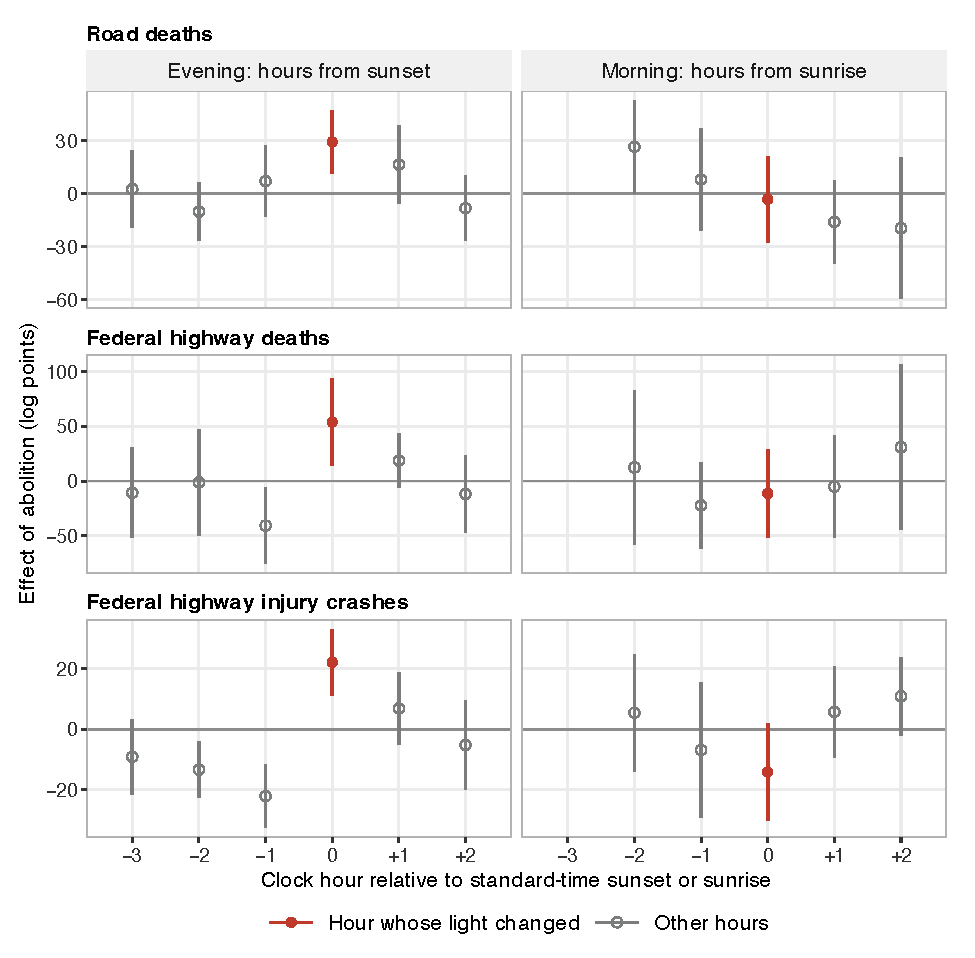
\includegraphics{fig_hours_from_sunset.pdf}
  \caption{Effect of Abolition by Hour Relative to Sunset and Sunrise}
  \label{fig:hours}
  \begin{figurenotes}[Notes]
  Each point is $\beta$ from Equation~(\ref{eq:main}) estimated separately for one clock hour, with its 95 percent confidence interval; standard errors clustered by state. Hour 0 is the 60 minutes after standard-time sunset (left) or sunrise (right), the hour that turned dark or light; hour $-1$ is the 60 minutes before.
  \end{figurenotes}
  \begin{figurenotes}[Sources]
  \citet{datasus2025sim}; \citet{prf2025dados}.
  \end{figurenotes}
\end{figure}

\subsection{Trends and robustness}\label{sec:trends}

\begin{figure}[tbp]
  \centering
  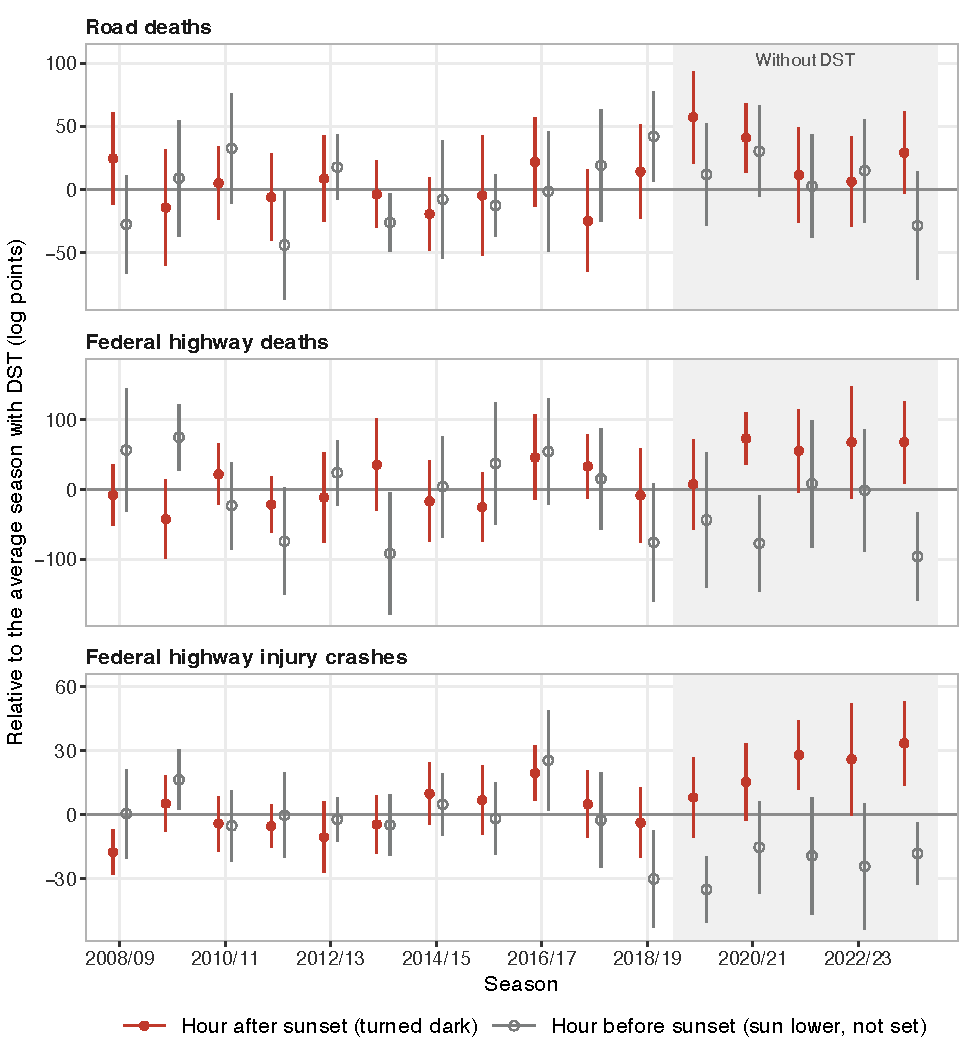
\includegraphics{fig_event_study.pdf}
  \caption{The Hour after Sunset and the Hour before, Season by Season}
  \label{fig:event-study}
  \begin{figurenotes}[Notes]
  Equation~(\ref{eq:main}) with $T_s W_d$ interacted with each season instead of with $A_d$, estimated with 2018/19 as the reference and shown against the average of the 11 seasons with DST, the comparison $\beta$ makes. 95 percent confidence intervals, standard errors clustered by state. The shaded seasons had no DST.
  \end{figurenotes}
  \begin{figurenotes}[Sources]
  \citet{datasus2025sim}; \citet{prf2025dados}.
  \end{figurenotes}
\end{figure}

Figure~\ref{fig:event-study} replaces the single post-abolition indicator with one coefficient per season, shown against the average season with DST, for hour 0 and the hour before it. For road deaths, the coefficients before abolition show no trend (a slope of $-0.5$ log points per season, standard error 2.1) and are jointly indistinguishable from each other ($p=0.18$). % pretrends.rds: pre_trend_lp, pre_trend_se, wald_pre_p.
All five seasons without DST lie above the average season with DST, the first two by the most. For federal highway injury crashes the earlier coefficients drift upward ($p<0.001$ for the joint test). In the hour before sunset, 2018/19 was already low relative to every earlier season, so the fall in that hour predates abolition. % switched_hour_event_study.rds: PRF injury crashes, hour -1, 2008/09-2017/18 between 24.9 and 55.5 log points against 2018/19.

\begin{table}[tbp]
  \caption{The Hour after Sunset under Other Choices, and Hours Whose Light Did Not Change}
  \label{tab:robustness}
  \centering\footnotesize\setlength{\tabcolsep}{5pt}
  \input{\tabdir/tab_robustness.tex}
  \begin{tablenotes}[Notes]
  Equation~(\ref{eq:main}) with one change per row; standard errors clustered by state. Panel A: the trend is fitted on all seasons. Without March 2020 to February 2022 drops every day of that period, which includes the off-season of 2019/20 from April to June 2020. The first and last summers come from one model with a separate effect for 2019/20 and 2020/21 and for 2021/22 to 2023/24. The summer-window row is a difference in differences, treated relative to control states and after relative to before, with state and date effects and no off-season. The joint test is a Wald test that the 11 season coefficients before abolition in Figure~\ref{fig:event-study} are equal. Panel B: counterfactual fitted on untreated state-days only, with week and day-of-week effects in place of date effects; 95 percent intervals in brackets, from 299 draws of a state bootstrap. Panel C: in the first row, the control states' events are counted, on each date, in the clock hour that starts at the treated states' standard-time sunset (average over their municipal seats, weighted by road deaths before abolition). The state-by-day row compares hour 0 with hours 3 to 5 before and 2 to 4 after sunset of the same state and day. The two-hour row counts events from standard-time sunset to two hours after it as one bin. Panel D: midday is at least three hours after sunrise and more than three hours before sunset; night is at least three hours after sunset or more than two hours before sunrise.
  \end{tablenotes}
  \begin{tablenotes}[Sources]
  \citet{datasus2025sim}; \citet{prf2025dados}.
  \end{tablenotes}
\end{table}

Table~\ref{tab:robustness} reports checks for these trends and other threats. With a linear treated-by-summer trend fitted on all seasons, the estimate for road deaths is 39.9 log points (20.7). That trend also runs through the seasons after abolition and can absorb part of the effect. Panel B instead uses a Poisson version of the imputation estimator of \citet{borusyak2024revisiting}, which fits the counterfactual on untreated observations. With a trend learned before 2019 and extrapolated, road deaths rose 38 percent (95 percent interval $-12$ to 103), compared with 31 percent (7 to 54) without the trend. The federal highway estimates are more sensitive to the trend. With the linear trend, the estimate for injury crashes falls from 22.2 to 5.6 log points (8.0); with the extrapolated trend, the imputation estimate falls from 23 to 8 percent ($-5$ to 26). We therefore rely on road deaths for the magnitude of the effect.

In the triple difference (Table~\ref{tab:robustness}, Panel A), the first two seasons without DST give 48.7 log points (11.6) and the last three 15.8 (10.3). The decline does not come from the summer window. Online Appendix Figure~\ref{fig:window-legs} splits the triple difference into its two legs, the gap between treated and control states in the summer window and the same gap in the off-season. In the summer window the gap rose with abolition and stayed up in all five seasons; estimated in the summer window alone, the effect is 39.3 (12.4) in the first two seasons and 31.2 (15.8) in the last three (Online Appendix Table~\ref{tab:sensitivity}). The off-season leg moved instead: it was low in 2019/20, whose off-season includes the pandemic months of April to June 2020, and high in 2021/22 and 2022/23. Dropping every day from March 2020 to February 2022 gives 22.9 (9.1); the summer window alone, with no off-season comparison, gives 34.5 (13.4) over all five seasons. Across these ways of handling the pandemic and the off-season, the estimate lies between 22.9 and 34.5 log points.

Federal highways also had a shock of their own in the first summer without DST: a presidential order suspended the use of the PRF's stationary, mobile, and portable speed cameras from mid-August to December 23, 2019 \citep{brasil2019despacho, poder3602019radares}. Without that summer, the federal highway estimates are larger (65.0 for deaths and 25.7 for injury crashes), and the estimate for road deaths, which include deaths on federal highways, is smaller (22.7, standard error 9.8; Online Appendix Table~\ref{tab:sensitivity}).

Although control states did not change their clocks, activities scheduled according to Bras\'ilia time occurred one hour earlier by local clock time during DST. This difference disappeared after abolition. Their evening traffic did not move, but their road deaths in hour 0 rose relative to the rest of the day; to the extent that this rise came from those schedules, the triple difference understates the effect. Within the treated states alone, the same comparison of hour 0 with hours of the same day yields 47.2 (7.8) (Online Appendix Table~\ref{tab:within-group}).

Other comparisons in Panel C of Table~\ref{tab:robustness} leave the estimate in the same range: counting the control states' deaths at the clock time of the treated states' hour 0 on each date, so that both groups are compared at the same time of the evening (33.3, 12.1); state-by-day fixed effects that compare hour 0 with hours of the same state and day whose light did not change (27.7, 12.4; season by season in Online Appendix Figure~\ref{fig:within-day}); leaving out Carnival and the year-end holidays (30.8, 8.0); and leaving out the 279 coastal municipalities \citep{ibge2022defrontantes}, the destinations of summer beach trips (36.3, 9.4; Online Appendix Table~\ref{tab:sensitivity}). Treating the two hours after sunset as one bin lowers the estimate to 21.2 (8.0): the second hour changed less, and adding it dilutes the estimate. No single state or season is decisive: leaving out one state at a time gives between 24.3 and 34.1, and one season at a time between 22.7 and 35.2 (Online Appendix Figure~\ref{fig:leave-out}). The control group matters more: with the eight states of the Northeast alone the estimate is 32.9 (9.2), with the four of the North alone 15.7 (8.8) (Online Appendix Table~\ref{tab:sensitivity}).

The sensitivity analysis of \citet{rambachan2023more} is less informative in this setting. Its target is the average post-abolition coefficient against 2018/19 (14.8 log points), not $\beta$, and with a single reference season that average is too imprecise to rule out small departures from a linear trend (Online Appendix Figure~\ref{fig:honestdid}). % honestdid.rds: avg_post_lp 14.85; breakdown M 0.02.
The case for a causal reading rests on the pattern within the day: the peak in one hour defined by the local sun, the smaller changes in the neighboring hours, the absence of a rise at midday and at night, whose light did not change, and the concentration among pedestrians.

Recorded times heap on the hour and the half hour (34.5 and 23.0 percent of road deaths), so whether a death falls in hour 0 can depend on how its time was rounded. Spreading each death recorded on the hour or half hour evenly over the 30 minutes around its recorded time gives 31.4 log points (9.5) in hour 0; dropping those deaths altogether leaves 16.7 (12.9), with less than half the sample. Moving the window by 5 to 15 minutes changes both how dark it is and which heaps of recorded times fall inside it. With the rounded times spread or dropped, the estimate rises at every step from a window that starts 15 minutes before standard-time sunset to one that starts 15 minutes after it, as an effect of darkness predicts (Online Appendix Figure~\ref{fig:window-shift}). Online Appendix Table~\ref{tab:measurement} collects these checks with those of Section~\ref{sec:data}.

\subsection{Darkness, not the clock}\label{sec:dose-results}

\begin{table}[tbp]
  \caption{Darkness as a Dose}
  \label{tab:dose}
  \centering\footnotesize\setlength{\tabcolsep}{5pt}
  \input{\tabdir/tab_dose.tex}
  \begin{tablenotes}[Notes]
  Estimates of $\theta_e$ (Panel A) and $\theta_m$ (Panel B) in Equation~(\ref{eq:dose}), on a panel of states, days, and the 24 clock hours, summer window and off-season; standard errors clustered by state. The dose of a clock hour is the change abolition brought to its darkness, with a minute of night counted as 1, a minute of civil twilight as one half, and a minute of daylight as 0, averaged over the state's municipal seats weighted by their road deaths before abolition. In the morning abolition moved hours from night toward daylight, so the doses there are negative; both panels report the effect of a clock hour going from full daylight to night. Every row has state-by-clock-hour-by-window and state-by-clock-hour-by-season effects. Date effects only: one effect per date, common to all clock hours. Baseline: one effect per clock hour and date. State-by-day effects: one per state and date added. Last row: one effect added for each clock hour in the treated states' summers after abolition. The permutation and score wild bootstrap $p$-values are computed for the baseline as in Table~\ref{tab:main}; in each permutation draw, the 11 states drawn as treated receive their own doses, and the test of equal evening and morning effects uses the $t$-statistic of their difference.
  \end{tablenotes}
  \begin{tablenotes}[Sources]
  \citet{datasus2025sim}; \citet{prf2025dados}; \citet{noaa2025solar}.
  \end{tablenotes}
\end{table}

An evening clock hour that goes from full daylight to night has 47.7 log points (9.7) more road deaths when the model includes an effect for every clock hour on every date (Equation~(\ref{eq:dose}) and Table~\ref{tab:dose}). With date effects common to all hours instead, the estimate is about the same (45.7, 6.3), so changes after 2019 at particular clock times across the country do not drive it. The last row adds a separate effect for every clock hour in the treated states' summers after abolition, which absorbs any change specific to those states at a given clock time. The dose effect is then identified by differences in darkness at the same clock hour, which arise because the sun sets at different clock times across the treated states and across the dates of the summer, and it is 52.3 (18.4). For the same change in darkness, the morning coefficient is $-6.4$ (14.7), which differs from the evening's ($p<0.001$; permutation $p=0.001$). The baseline evening effect remains significant under the permutation test ($p=0.002$) and the score wild bootstrap ($p<0.001$). On federal highways, deaths respond too (79.5, 20.6), and injury crashes less (13.6, 9.0). Pedestrians respond most: a fully dark evening hour raises their road deaths by 115.8 log points (29.7), compared with 33.6 (11.9) for everyone else. % light_dose.rds: inference; dose (SIM pedestrian and non-pedestrian deaths, spec main).

\subsection{Is it sleep?}

Two features of the design keep acute sleep loss out of the estimates: abolition involved no lost night, and the summer window excludes the weeks after clock changes. A chronic effect through the clock time of sunset \citep{giuntella2019sunset} would run the other way, since an earlier clock sunset should lengthen sleep, not shorten it. And a sleep effect would not confine itself to one hour of the day. Panel D of Table~\ref{tab:robustness} estimates Equation~(\ref{eq:main}) for hours whose light did not change, midday and night. Nothing rises in them: road deaths move by $-4.5$ (5.8) and $-6.6$ (5.6) log points. The design can detect such changes: deaths from assault, examined the same way, jump in 2019/20 alone, over the whole day as well as in the early evening (Online Appendix Figure~\ref{fig:assault}). Federal highway injury crashes fall at night ($-6.1$, $p=0.04$), consistent with the traffic that left the dark evening (Section~\ref{sec:traffic}).

\subsection{Who dies}

\begin{table}[tbp]
  \caption{Pedestrians and Other Road Users in the Hour after Sunset}
  \label{tab:pedestrians}
  \centering\footnotesize
  \input{\tabdir/tab_pedestrians.tex}
  \begin{tablenotes}[Notes]
  Equation~(\ref{eq:main}) for hour 0, estimated separately for events with a pedestrian victim and for all others; Panel C from one stacked model. Inference as in Table~\ref{tab:main}, with the wild cluster bootstrap $p$-value from the linear model; in each permutation draw both members of the pair receive the same set of treated states, and the difference is divided by the square root of the sum of the two squared standard errors. Excess events are observed minus predicted without abolition, treated states, summer window, after 2019; the pedestrian share of the excess has a delta-method standard error in parentheses.
  \end{tablenotes}
  \begin{tablenotes}[Sources]
  \citet{datasus2025sim}; \citet{prf2025dados}.
  \end{tablenotes}
\end{table}

The increase falls disproportionately on pedestrians (Table~\ref{tab:pedestrians}). Pedestrian road deaths in hour 0 rose by 76.6 log points (29.8), more than doubling, while the deaths of all other road users rose by 17.9 (7.8). Pedestrians were 11.7 percent of road deaths in hour 0 before abolition and account for 43.4 percent of the excess after it (standard error 10.3). On federal highways the contrast is sharper: 170 log points for pedestrian deaths and 26 for all others. The pedestrian estimates are significant under the wild bootstrap and the permutation test in all three outcomes. The difference between pedestrians and others is significant on federal highways (permutation $p=0.001$ for deaths and for injury crashes) and borderline for road deaths ($p=0.075$). The federal highway contrast does not come from their trend: with a pre-abolition trend extrapolated, pedestrian deaths there rise by 103.9 log points (34.3) and other deaths by 15.3 (23.5). % mechanism.rds, trend: extrap_lp for PRF pedestrian and non-pedestrian deaths.

Among the other road users (Online Appendix Table~\ref{tab:road-users}), motorcyclist deaths rose by 19.6 log points (10.9), and the estimate for car occupants is zero but imprecise ($-0.2$, standard error 35.2); deaths in the residual group, 85 percent of them with no type of vehicle recorded, rose by 55.8 (26.4). The ordering among pedestrians, motorcyclists, and car occupants is the one visibility predicts. A pedestrian is the road user who most depends on being seen, and pedestrian crash risk is the most sensitive to ambient light around the clock changes \citep{sullivan2002role, woods2025daylight}; pedestrian deaths at night also fall on brighter moonlit nights \citep{tyndall2025road}. The pattern is also hard to reconcile with sleep, which would impair drivers whoever they hit. The increase was larger on weekends and holidays (41.3, 15.8) than on weekdays (16.1, 10.0), and remains so when Carnival and the year-end holidays are excluded (39.3, 16.2), so it is not confined to the commute home. Among men, about four fifths of the dead, road deaths rose by 33.8 log points (9.9) and federal highway deaths by 65.2 (20.7); for women the estimates are too imprecise to compare (Online Appendix Table~\ref{tab:sex-age}; \citealp{prf2025pessoas}).

If the increase comes from darkness, it should be smaller where streets are lit. The 2022 Census, taken during the seasons without DST, records for each block face whether it has street lighting \citep{ibge2023censo}. We split the municipalities of each state at the median share of households on block faces without it (Online Appendix Table~\ref{tab:lighting}). In hour 0 the estimate for road deaths is 42.5 log points (10.0) in municipalities above the median, where streets are darker, and 10.9 (16.0) in those below it. The difference has the expected sign but is imprecise ($p=0.10$). Lighting measured in the 2010 Census, nine years before abolition and for urban tracts only, gives a smaller gap in the same direction (37.1 and 22.9, $p=0.61$; \citealp{ibge2011censo}). The two groups of municipalities may also differ in ways other than lighting. The pattern is therefore consistent with a role for street lighting, and does not establish one.

\subsection{Traffic followed the light}\label{sec:traffic}

We estimate Equation~(\ref{eq:main}) on hourly vehicle counts at federal highway stations (Online Appendix Table~\ref{tab:volume}). After abolition, traffic in the treated states' summer fell by 6.4 log points (2.2) in hour 0 and by 5.1 (1.3) in the hour before it, and rose by 11.7 (5.0) in the morning hour that turned light, with permutation $p$-values of 0.069, 0.025, and 0.159. None of the stations counted after abolition had been counted before it: counting resumed in 2021 under a new contract, at new stations (Section~\ref{sec:data}). On the 30 stations that were moved at most 2 kilometers along the same highway, the evening fall is smaller and not significant ($-3.1$, 3.1) and the morning rise larger (18.7, 5.1).

Subtracting the volume estimate from the crash estimate gives the change in crashes per vehicle. For a like-for-like comparison, the crash estimates in that table come from the summers covered by the traffic counts, 2014/15 to 2018/19 and 2021/22 to 2024/25, over which federal highway injury crashes in hour 0 show no trend before abolition ($-2.8$ log points per season, standard error 2.9). % traffic_volume.rds, risk: pre_trend_lp, PRF injury accidents, eve+0.
On those summers, injury crashes in hour 0 rose by 17.6 log points (7.5), and injury crashes per vehicle by 24.0 ($p=0.005$), more than crashes themselves; in the morning hour that turned light, crashes per vehicle fell by 28.1 ($p=0.083$). Fewer vehicles travel in hour 0, and each faces a higher risk. The stations cover federal highways only and say nothing about urban traffic, where many of the pedestrian deaths in the death registry occur.

\subsection{The morning hour does not offset the evening hour}\label{sec:offset}

\begin{table}[tbp]
  \caption{Excess Events per Summer after Abolition}
  \label{tab:excess}
  \centering\footnotesize
  \input{\tabdir/tab_excess.tex}
  \begin{tablenotes}[Notes]
  Events per summer in the treated states after abolition minus those predicted without it; delta-method standard errors in parentheses, from coefficients with standard errors clustered by state. Panel A: Equation~(\ref{eq:dose}), baseline of Table~\ref{tab:dose}, summed over every clock hour of the summer window; the whole DST season applies the same coefficients to the days of the season under the 2017 rule (first Sunday of November to third Sunday of February) outside the window; the row below it refits the model with a separate dose effect for November 15 to December 7, for December 24 to January 15, and for the other days of the window, and applies the effect of November 15 to December 7 to the days outside the window. Evening and morning hours may not add to the net because of rounding. Panel B: one model that stacks seven hours (two before to two after standard-time sunset; one before to two after standard-time sunrise) with every fixed effect of Equation~(\ref{eq:main}) interacted with the hour; the whole day comes from a separate model. Panel C: observed events in each hour times $1 - e^{-v}$, where $v$ is the change in that hour's federal highway traffic (column 1 of Online Appendix Table~\ref{tab:volume}, every hour and the rest of the day in one model); the hours whose light changed are the two after sunset and the hour before and after sunrise. Only events with a recorded clock time, so the counts understate the events in each hour. The clustered $p$-value of the net count uses its delta-method standard error. The permutation $p$-value of the net count compares its ratio to its delta-method standard error with the same ratio in 999 draws of 11 treated states, each with its own doses. The net count is a nonlinear function of both coefficients, so it has no restricted model for the score wild bootstrap and no linear analogue for the wild cluster bootstrap of Table~\ref{tab:main}.
  \end{tablenotes}
  \begin{tablenotes}[Sources]
  \citet{datasus2025sim}; \citet{prf2025dados}; \citet{dnit2025pnct}.
  \end{tablenotes}
\end{table}

Table~\ref{tab:excess} turns the estimates into events per summer: observed counts in the treated states' summers after abolition minus those predicted without it. Panel A sums every clock hour of the day, weighted by how much darker or lighter it became (Equation~\ref{eq:dose}). Abolition added 62 road deaths per summer window (standard error 12; permutation $p=0.001$): 57 in the evening hours that grew darker, and 5 in the morning hours that grew lighter, where the effect is indistinguishable from zero. Extended to a full DST season under the 2017 rule, about 108 days instead of the 92 of the window, the estimate yields 74 additional deaths (standard error 14). This extension applies coefficients estimated within the summer window to days outside it. The count requires no selection of particular hours, but it assumes that hours with no change in the modeled darkness dose were unaffected. A dose of zero does not mean that the light did not change at all: the hour before standard-time sunset stayed in daylight, with the sun lower. Panel D of Table~\ref{tab:robustness} finds no detectable change at midday or at night. Each of these blocks had only about 580 road deaths with a recorded time per summer window in the treated states before abolition, so their confidence intervals also include a fall as large as the net count. % placebo_hours.rds: 585 and 572 per season; 95 percent intervals about -86 to +42 and -93 to +26 deaths.

Panel B adds up hours estimated one at a time, without that structure. The two evening hours that turned darker added 57 road deaths per summer (standard error 19), and the morning hour that turned light removed 3 (11). That hour gained traffic along with light: on federal highways its vehicles rose by about 12 percent and its injury crashes per vehicle fell by 28 log points (Section~\ref{sec:traffic}), so a lower risk per trip was spread over more trips. Together, these three hours added a net 54 deaths (20), 17 percent of the deaths predicted in them ($p=0.007$). % reallocation.rds, sums: 54.23, se 20.06, pct_of_cf 17.3, p 0.0069.
Hours $-1$ to $+1$ at each end, from one hour before to two hours after sunset and sunrise, give 53 (35), and all seven hours 41 (41). Estimated directly, the whole day gives $-5$ deaths (66). Estimating the effect over the entire day introduces variation from hours in which the effect is small or absent, making the net estimate considerably less precise than the evening-hour estimate. The whole-day count can therefore neither confirm the net figure nor rule it out, and we do not read it as evidence that abolition only moved deaths between hours of the day. On federal highways, the dose model implies 31 deaths (12; permutation $p=0.135$) per summer; injury crashes, whose response to darkness is weaker, net 43 (57).

An offset would require deaths to fall in the hours whose light did not change, the reallocation across hours that \citet{james2023let} finds in Australia. The most direct mechanism for such an offset would be trips moved out of the hours whose light did not change. In Panel C of Table~\ref{tab:excess}, we compute the deaths that the change in federal highway traffic would imply in each hour if the risk per vehicle had stayed the same. Traffic fell in the evening hours adjacent to hour 0 and changed by 2.6 log points (standard error 2.0) over the rest of the day. In the hours whose light did not change, the implied change is an increase of 15 road deaths per summer (standard error 32). Its 95 percent confidence interval, from a decline of about 47 deaths to an increase of about 77, excludes a decline as large as the net count of 62 but not a partial offset of up to about three quarters of it. For federal highway deaths, which the stations cover, the implied change is 7 (12), compared with a net count of 31. In the hours whose light changed, the traffic alone would imply 4 fewer road deaths (standard error 15), so the increase in those hours came from a higher risk per trip, not from more trips. This calculation addresses only offsets that arise from changes in when people travel, not changes in the risk of a trip. Nor does it cover urban streets, where many pedestrian deaths occur, because the stations count only federal highways.
% total_cost.rds, implied: light unchanged, SIM 15.1 (31.6; 95 percent interval -46.8 to 77.0), PRF deaths 7.2 (12.5); light changed, SIM -4.3 (14.9); implied_hours: rest vol_lp 2.60 (2.03).

In levels, a clock hour that goes from full daylight to night has about 61 percent more road deaths, and more than three times as many pedestrian deaths. That pedestrians bear so much of the increase matches evidence that their crash risk in the dark is up to seven times that in daylight \citep{sullivan2002role}. The effect on all road users is larger than projections for the United States. Over the three hours of Panel B of Table~\ref{tab:excess}, abolition added 17 percent to the predicted road deaths, while \citet{coate2004effects} project that year-round DST would lower deaths in the morning and evening periods it affects by 13 percent for pedestrians and 3 percent for vehicle occupants.
\subsection{Before and after travel adjusted}\label{sec:transitions}

The clock changes before 2019 produced the same change of light as abolition, before travel had time to adjust. When the clocks went back each February, the evening hour 0 went from daylight to dark overnight, while work, school, and travel kept to the same clock hours; when they went forward each spring, the reverse. Online Appendix Table~\ref{tab:transitions} compares hour 0 in the three weeks after each change with the three weeks before, in the treated relative to the control states, and uses the same calendar days of the seasons after abolition, when no clock moved, to net out the seasonal change. In the three weeks after the clocks went back, road deaths in hour 0 rose by 54.6 log points (21.9); after they went forward, deaths fell by 29.9 (18.5). Read as the effect of a darker evening, the two average 42.3 (13.8), compared with 29.2 after abolition. On federal highways the same comparison implies 121 log points for deaths at the clock changes and 54 after abolition, and about the same for injury crashes (20.6 and 22.2). Each change also adds or removes an hour of sleep, which acts on every hour of the day and pushes both transition estimates toward zero; compared with hours of the same day, which nets it out, the transitions give 79.1 (14.2) and abolition 27.7 (12.4). In one model that allows for the overlap of the two samples, abolition minus the clock changes is $-13.1$ (12.5) in the first comparison and $-51.4$ (18.3) in the second. For road deaths, only the within-day comparison, which absorbs day-level shocks common to all hours, including those associated with sleep, yields a statistically significant difference between the transition and abolition estimates.

The two settings also differ in the time of year, and the effect of abolition is not the same across the summer window (Online Appendix Table~\ref{tab:window-parts}). From November 15 to December 7, while schools are in session, abolition raised road deaths in hour 0 by 58.1 log points (12.6). From December 24 to January 15 it is $-12.3$ (16.8). From January 16 to 31 it is 49.1 (15.6), although schools are still on break then in every treated state but Goi\'as \citep{saopaulo2018resolucao, goias2018parecer, minas2023ano}. The school calendar alone therefore cannot explain how the estimate varies across the summer window. Before abolition the parts of the window moved alike (Online Appendix Table~\ref{tab:window-parts}). Federal highway traffic shows no detectable difference between the weeks from Christmas to mid-January and the school weeks, whether counted in hour 0, for trucks and buses alone, or over the whole day (Online Appendix Table~\ref{tab:traffic-parts}). These checks do not rule out holiday travel on other roads as an explanation, and the data do not say why no increase is detectable from Christmas to mid-January.

The three weeks after each clock change fall while schools are in session, the same part of the school year as the weeks from mid-November to early December. Compared with abolition in those weeks, the clock changes are not distinguishable from it: the difference is 15.8 (18.0) in hour 0 and $-22.2$ (20.9) in the comparison with hours of the same day (Online Appendix Table~\ref{tab:transitions}). The gap over the whole window thus points mainly to the weeks from Christmas to mid-January rather than to a uniformly smaller effect after travel adjusted, though the intervals leave room for a moderate decline.

% -----------------------------------------------------------------------------
\section{What Abolition Cost}\label{sec:cost}

\begin{table}[tbp]
  \caption{Deaths per Summer and What They Are Worth}
  \label{tab:cost}
  \centering\footnotesize
  \input{\tabdir/tab_cost.tex}
  \begin{tablenotes}[Notes]
  Panel A: net excess deaths over every hour of the day from the darkness dose model (Table~\ref{tab:excess}, Panel A), in the summer window and over the whole DST season under the 2017 rule. Column 1 is the estimate. Column 2 adds road deaths without a clock time, assuming they occur in the affected hours in the same proportion as deaths with one. Column 3 adds deaths off the road, 85 percent of them in hospitals, under the same assumption; it is an extrapolation. The share is of all land-transport deaths in the treated states' summer window before abolition. The whole-season count applies coefficients estimated in the summer window to the additional days covered by the 2017 DST rule. Panel B: the summer-window counts valued at the value of a statistical life (VSL) by the reference approach of \citet{robinson2019valuing} and two alternatives, from gross national income per head at purchasing-power parity in 2025, in international dollars; and the Ipea social cost of a death on a federal highway, a human-capital cost that excludes the value of life itself (December 2014 prices adjusted to December 2025 prices using the IPCA and converted at the 2025 PPP rate of 2.554 reais per international dollar). Panel C: the whole-season counts at the reference VSL. Delta-method standard errors in parentheses, from coefficients with standard errors clustered by state.
  \end{tablenotes}
  \begin{tablenotes}[Sources]
  \citet{worldbank2026wdi}; \citet{ipea2015acidentes}; \citet{ibge2026ipca}.
  \end{tablenotes}
\end{table}

Table~\ref{tab:cost} scales and values the net count of the dose model. Column 1 reports the estimated increase in road deaths with a recorded time: 62 deaths per summer window and 74 when extended to the full DST season (Table~\ref{tab:excess}). Both counts assume, as discussed in Section~\ref{sec:offset}, that hours with no change in the modeled darkness dose were unaffected. The full season is the relevant unit for the policy choice, since reinstating DST would restore all of it. The figure of 74 deaths is obtained by applying the average effect of the summer window to the extra days, in early November and mid-February; that average includes the weeks from Christmas to mid-January, when no increase was detectable (Section~\ref{sec:transitions}). Refitting the dose model with a separate effect for each part of the window and applying the effect of November 15 to December 7 to the extra days yields 79 deaths (Table~\ref{tab:excess}). Early November falls in the same part of the school year as November 15 to December 7; mid-February, when many school systems are reopening, may be closer to the smaller estimate for February 1 to 14. Because the extra days lie outside the estimation window, 79 is a sensitivity calculation. % light_dose.rds, dose: season_net_term 78.8 (SIM, main).
 The summer-window deaths are 1.0 percent of all land-transport deaths in the treated states' summer window. Column 2 assumes that road deaths without a recorded time fall in the affected hours in the same proportion as those with one, which gives 77 per summer window. Column 3 further assumes that deaths occurring off the road, 85 percent of them in hospitals, follow the same hourly pattern as deaths at the crash scene, yielding 157 deaths per summer window. This is an extrapolation: the design cannot identify the crash hour for in-hospital deaths. The resulting bias could run in either direction, because pedestrians struck in darkness may be more or less likely than other crash victims to die at the crash scene.

We value a death with the reference rule of \citet{robinson2019valuing} for transferring a value of a statistical life (VSL) to a lower-income country: the US ratio of VSL to income per head, 160, extrapolated to Brazil with an income elasticity of 1.5, so that $\mathit{VSL}_{\mathit{BR}} = 160\, Y_{\mathit{US}}\, (Y_{\mathit{BR}}/Y_{\mathit{US}})^{1.5}$, where $Y$ is gross national income per head at purchasing power parity in 2025 \citep{worldbank2026wdi}. The resulting VSL is 1.8 million 2025 international dollars, or R\$4.7 million at the 2025 parity rate (Online Appendix~\ref{app:cost} gives the inputs and the alternative rules).  % total_cost.rds, vsl: 1,825,618 international dollars; R$ 4.66338 million.
The deaths in each summer window add up to an estimated cost of 114 million international dollars (standard error 22), rising to 287 million under the broadest scaling; over a whole season of DST, the deaths in column 1 cost 135 million. If the summer-window count is set at the lower end of its 95 percent confidence interval, 39 deaths, the cost is 71 million. For the two evening hours and the morning hour estimated one at a time (Panel B of Table~\ref{tab:excess}), whose sum does not impose the dose model's weighting of hours, the lower end is 15 deaths, or 27 million. The two alternative rules of \citet{robinson2019valuing} give larger values, up to 571 million per summer window. A human-capital valuation of a death on a federal highway \citep{ipea2015acidentes}, which leaves out the value of life itself, gives 19 to 49 million. The valuation counts deaths only, so it leaves out two costs. First, we do not estimate the quality-adjusted life years (QALYs) lost by people who were injured and survived. Injury crashes on federal highways rose too, but the death registry does not record injuries, and the federal highway estimate is sensitive to its trend. Second, we do not value avoidance: traffic in the hour that turned dark fell, consistent with trips moved or forgone, but the data do not show who changed their travel or at what cost. The deaths are the harm that remained after that avoidance.
% total_cost.rds, value: DST season, count A, rule (a): 134.7 (se 26.3).
% total_cost.rds, lower: lo95 38.8 (71 million), three hours 14.9 (27 million).

For comparison, the national grid operator projects that reinstating DST would save 96 to 139 million international dollars in thermal-generation fuel from October 2024 to February 2025, of the same order as the cost of the deaths in a DST season (135 million), and about 0.7 billion a year in payments for reserve capacity \citep{ons2024nota}. % ONS reais (R$244-356 million; R$1.8 billion) converted at the 2025 PPP factor, 2.55441.
Reinstating DST would also restore the two clock changes a year that abolition removed, whose cost the literature attributes to lost sleep in the days after the spring change: more road crashes \citep{smith2016spring, gillmore2025daylight} and, in Brazil, more deaths from heart attacks \citep{toro2015daylight}. Section~\ref{sec:transitions} compares the clock changes with abolition, but the summer window excludes those weeks, and the valuation here does not include them.

% -----------------------------------------------------------------------------
\section{Conclusion}\label{sec:conclusion}

When Brazil stopped moving its clocks, the evening hour that lost its sunlight became deadlier on the road, disproportionately for pedestrians, and the morning hour that gained light did not become detectably safer. When only deaths at the crash scene with a recorded time are counted, and hours that remained in full daylight or full darkness are assumed unaffected, abolition of DST added 62 road deaths from mid-November to mid-February each year, and about 74 if the effect is extended to the rest of the season. The increase was detectable from mid-November to early December and in late January, but not from Christmas to mid-January. In the first of these periods it was statistically indistinguishable from the effect at the clock changes, when travel had no time to adjust.

The estimates have limits that matter for their use. They count only deaths at the crash scene with a recorded time, not deaths off the road or without a recorded time, nor nonfatal injuries. The sample has 23 states and five summers without DST, two of them in the pandemic; the estimate lies between 23 and 34 log points across the ways of handling the pandemic and the off-season, and in the summer comparison it shows no clear decline over the five seasons. The net count over the day assumes that hours with no change in the modeled darkness dose were unaffected; estimated without that restriction, the whole-day effect is too imprecise to say whether some deaths moved to other hours. Federal highway records are sensitive to a pre-existing trend, and the traffic counts cover only federal highways.

For Brazil, the estimates speak to the choice between reinstating seasonal DST and maintaining year-round standard time. At the reference value of a statistical life, the crash-scene deaths with a recorded time cost an estimated 114 million 2025 international dollars per summer window. The estimates are less directly transferable to other settings. In summer, seasonal and permanent DST set the same clock, so the estimates are the cost, in summer evenings, of choosing permanent standard time over either. They say nothing about winter, when permanent DST would darken the mornings, and they are least informative at latitudes higher than Brazil's. Nor do they weigh the clock changes, energy use, or the effects of the clock on sleep. Part of what people did to protect themselves, driving less in the hour that turned dark, is already in the estimates. Pedestrians account for a disproportionate share of the additional deaths, and street lighting and road design may protect them when the clock does not.


% References start on a new page, after every float of the text.
\clearpage
\bibliographystyle{aea}
\bibliography{references}

\clearpage
\appendix
\setcounter{page}{1}
\renewcommand{\thepage}{A\arabic{page}}
\begin{center}\Large\textbf{Online Appendix}\end{center}
\makeatletter
\@addtoreset{figure}{section}\@addtoreset{table}{section}
\renewcommand{\thefigure}{\thesection\arabic{figure}}
\renewcommand{\thetable}{\thesection\arabic{table}}
\makeatother
% =============================================================================
% appendix_body.tex: the Online Appendix. Read by appendix.tex (submitted as a
% separate, anonymized file) and by paper_wp.tex (appended to the working
% paper). Sections are lettered and exhibits numbered within them (Figure A1,
% Table B1, ...). Numbers come from the generated exhibits or from audit/*.rds,
% as in body.tex.
% =============================================================================

\section{Data and Measurement}\label{app:data}

The main outcome assigns road deaths to clock hours using the times recorded on their death certificates. Table~\ref{tab:measurement} summarizes the evidence on the reliability of this assignment: the correspondence between recorded crash and death times, the stability of reporting across abolition, the concentration of recorded times at whole and half hours, and the sensitivity of the estimates to shifted time windows and alternative treatments of rounded times. The subsections below describe each check.

\begin{table}[tbp]
  \caption{Measuring the Hour of Death}
  \label{tab:measurement}
  \centering\footnotesize\setlength{\tabcolsep}{5pt}
  \input{\tabdir/tab_measurement.tex}
  \begin{tablenotes}[Notes]
  Panels A and B use the death register only. Panel A: each federal highway crash with one death is paired with the only road-death certificate with a clock time in the same municipality on the same date. As a benchmark for chance, the crash is also paired with the certificates of the same municipality seven days later, which cannot record the same death. Panel B: linear triple difference on each share by state, season and window, weighted by deaths, with state-by-window, state-by-season and season-by-window effects. Panel D: equation~(\ref{eq:main}) for hour 0, one change per row; the window rows start the 60-minute window that many minutes before or after standard-time sunset; spread: full- and half-hour times spread over the 30 minutes around them; the last row takes sunset from the full NOAA solar algorithm \citep{meeus1998astronomical}. Standard errors clustered by state.
  \end{tablenotes}
  \begin{tablenotes}[Sources]
  \citet{datasus2025sim}; \citet{prf2025dados}.
  \end{tablenotes}
\end{table}

\subsection{The legal calendar}

The dates and states of DST come from the decrees themselves, typed from the texts published by the Presidency \citep{brasil2008decreto, brasil2017decreto, brasil2019decreto}. Under Decree 6,558/2008, DST ran from midnight on the third Sunday of October to midnight on the third Sunday of February, a week later when that Sunday was Carnival Sunday (as in 2012 and 2015); Decree 9,242/2017 moved the start to the first Sunday of November from 2018. Within the sample, DST therefore started between 15 October and 4 November and ended between 15 and 26 February. A day is under DST when the start date is on or before it and the end date is after it, since both changes happen at midnight. Decree 7,584/2011 added Bahia for 2011/12; Decree 7,826/2012 removed Bahia and added Tocantins for 2012/13, and Decree 8,112/2013 removed Tocantins. Decree 9,772/2019 abolished DST in the whole country and revoked the decrees still in force, 6,558/2008, 8,112/2013 and 9,242/2017 among them.

\subsection{Deaths on the road}

Road deaths are deaths whose underlying cause is a land-transport accident (ICD-10 V01--V89) and whose place of occurrence is a public road. Pedestrians are V01--V09; cyclists V10--V19; motorcyclists V20--V29; occupants of cars and light vehicles V40--V59; the remaining codes are other road users. The clock time is the time of death written on the certificate, in hours and minutes; times that are missing or invalid are left out of every hourly count. Figure~\ref{fig:records} shows, for the summer window, the share of land-transport deaths that occurred on the road and the share of road deaths without a valid clock time, by group and season. A linear triple difference on each share, computed by state, season and window and weighted by deaths, with state-by-window, state-by-season and season-by-window fixed effects, gives $+0.4$ percentage points (standard error 0.75) for the share on the road and $+0.4$ (0.65) for the share without a time (Table~\ref{tab:measurement}, Panel B). % record_integrity.rds, test.

The time on the certificate is close to the time of the crash for deaths at the scene. Pairing each federal highway crash with one death with the only road-death certificate with a clock time in the same municipality and on the same date gives 37,875 pairs, most of them the same event. The certificate's time minus the crash time has a median of zero minutes; it lies in the hour after the crash in 59.2 percent of the pairs and within 30 minutes either way in 66.9 percent. Pairs formed with the certificates of the same municipality seven days later, which cannot be the same event, give 4.7 and 5.2 percent (Table~\ref{tab:measurement}, Panel A). % record_integrity.rds, link.

Death certificates record legal clock time. If they recorded standard time, the profile of road deaths by clock hour in the treated states' summers under DST would sit one hour earlier than without DST. Net of the off-season and of the control states, the two profiles are closer with no shift (squared distance 7.8) than with a shift of one hour in either direction (17.1 and 24.5). % record_integrity.rds, clock.

\begin{figure}[tbp]
  \centering
  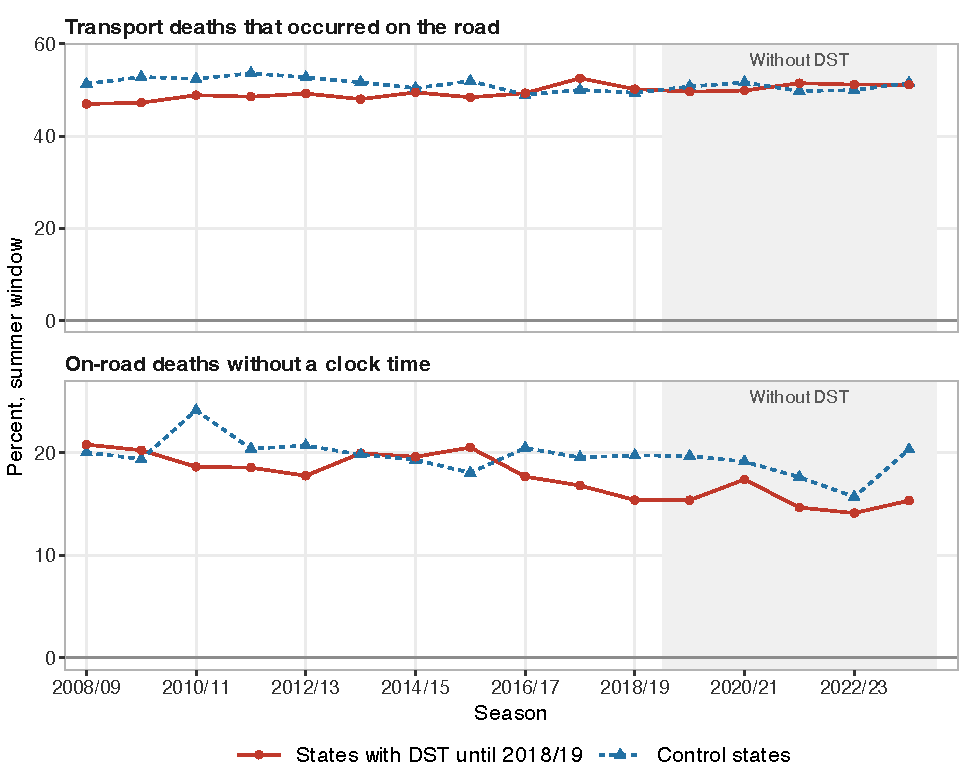
\includegraphics{fig_record_integrity.pdf}
  \caption{How Road Deaths Are Recorded}
  \label{fig:records}
  \begin{figurenotes}[Notes]
  Land-transport deaths (V01--V89) in the summer window. Top: share that occurred on the road rather than in hospital or elsewhere. Bottom: share of road deaths without a valid clock time.
  \end{figurenotes}
  \begin{figurenotes}[Source]
  \citet{datasus2025sim}.
  \end{figurenotes}
\end{figure}

\subsection{Federal highway crashes}

The PRF files have one row per crash from 2007 to 2025. Date formats, text encodings and the case of the light-phase labels change across years and are harmonized; a crash that appears on several rows differing only in a descriptive field is kept once. The municipality is given by name and is matched to the IBGE code within the state, with a table of alternative spellings and renamed municipalities typed by hand and checked against the coordinates that the PRF reports from 2017; every crash is matched. The light phase recorded by the officer is one of full daylight, dawn, dusk and night; in Panel B of Figure~\ref{fig:light} and in the first stage, dusk and night count as dark, and dawn crashes are left out. A second set of PRF files has one row per person in each crash, with the person's role, condition, sex and age \citep{prf2025pessoas}; matched to the crashes by their identifier, its dead match the deaths of the crash files to within one in every year of the sample, and it gives the sex and age of the dead in Table~\ref{tab:sex-age}.

\subsection{Traffic counts}

The counts are hourly vehicles by direction and vehicle class at continuous counting stations. A station-day enters only if all 24 clock hours are present and the daily total is positive. Each hourly count is assigned to the 60-minute bin, relative to standard-time sunset or sunrise at the station, that contains the midpoint of its clock hour. The flag for modeled values marks a station-day whose daily total equals exactly that of the same weekday one to four weeks earlier or later; such repetitions are absent from counts before June 2019 and frequent after it at the stations whose published values DNIT estimated. Of the stations in the 23 states of the sample, 247 report only before abolition and 315 only after. % EXPLICANDO_O_PROJETO.md, section 3.3 (count corrected in the code audit of 09/10/2026).

The stations record legal clock time. If they recorded standard time, the profile of traffic by clock hour in the treated states' summers under DST would sit one hour earlier than without DST. Net of the off-season and of the control states, the two profiles are closer with no shift (squared distance 0.23) than with a shift of one hour in either direction (0.32 and 0.38). % traffic_volume.rds, clock.

\subsection{Sun times and recorded times}

Sunrise and sunset are computed at the municipal seat \citep{noaa2025solar}, with the seat coordinates from IBGE (2010 seats; a point inside the 2020 boundary for the five municipalities created in 2013) and the standard offset of each municipality's legal time zone \citep{brasil1913decreto, brasil2008lei, brasil2013lei}. Recorded clock times heap: 34.5 percent of road deaths are recorded on the full hour and 23.0 percent on the half hour, and 90 percent on a multiple of five minutes (21.3, 19.4 and 95.2 percent for federal highway deaths). % heaping.rds, heap_share.
Because hour 0 is defined relative to the sunset of each municipality and date, a heap at, say, 7:00 p.m.\ falls inside or outside hour 0 depending on the place and the date. Figure~\ref{fig:window-shift} and Panel D of Table~\ref{tab:measurement} show the estimates when the window is moved by up to 15 minutes, when sunset comes from NOAA's full solar algorithm \citep{meeus1998astronomical} instead of the general equations, when every time recorded on the full or half hour is spread evenly over the 30 minutes around it, and when those times are dropped.

% -----------------------------------------------------------------------------
\section{Additional Results}\label{app:results}

\subsection{Other windows, samples and clocks}

\begin{figure}[tbp]
  \centering
  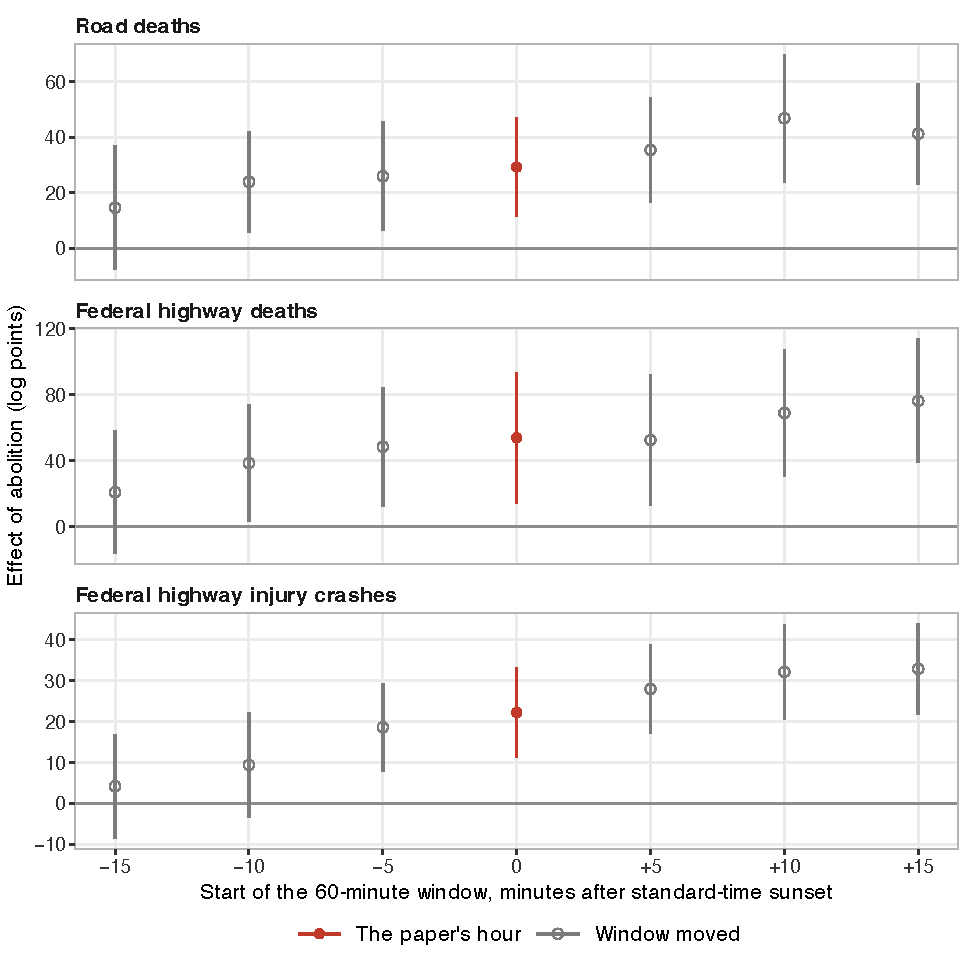
\includegraphics{fig_window_shift.pdf}
  \caption{The Hour after Sunset, Moved Earlier and Later}
  \label{fig:window-shift}
  \begin{figurenotes}[Notes]
  Each point is equation~(\ref{eq:main}) for a 60-minute window that starts the stated number of minutes after standard-time sunset; 0 is hour 0 of Table~\ref{tab:main}. 95 percent confidence intervals, standard errors clustered by state.
  \end{figurenotes}
  \begin{figurenotes}[Sources]
  \citet{datasus2025sim}; \citet{prf2025dados}.
  \end{figurenotes}
\end{figure}

\begin{figure}[tbp]
  \centering
  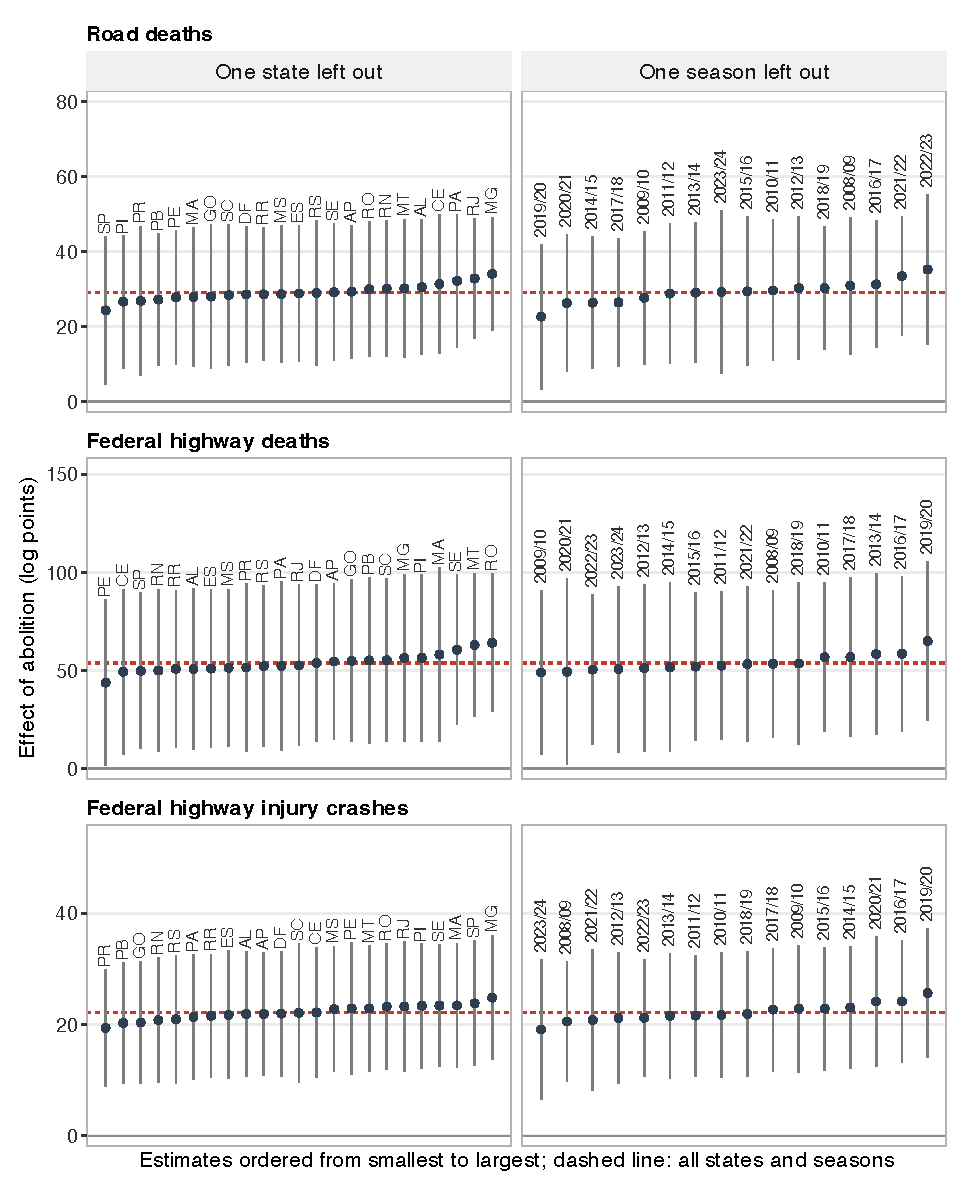
\includegraphics{fig_leave_out.pdf}
  \caption{Leaving One State or One Season Out}
  \label{fig:leave-out}
  \begin{figurenotes}[Notes]
  Equation~(\ref{eq:main}) for hour 0, dropping the state or season named above each point. 95 percent confidence intervals, standard errors clustered by state; the dashed line is the estimate with every state and season.
  \end{figurenotes}
  \begin{figurenotes}[Sources]
  \citet{datasus2025sim}; \citet{prf2025dados}.
  \end{figurenotes}
\end{figure}

\begin{table}[tbp]
  \caption{The Hour after Sunset under Other Samples}
  \label{tab:sensitivity}
  \centering\footnotesize\setlength{\tabcolsep}{5pt}
  \input{\tabdir/tab_sensitivity.tex}
  \begin{tablenotes}[Notes]
  Equation~(\ref{eq:main}) for hour 0, one change per row, standard errors clustered by state. Panel A: the coast row drops the events in the 279 municipalities that face the sea \citep{ibge2022defrontantes}; the holiday row drops Saturday before Carnival to Ash Wednesday and 24 December to 1 January. The summer-window rows are the difference in differences of Table~\ref{tab:robustness} with separate effects for the first two and the last three summers without DST. The rows without March 2020 to February 2022 have separate effects for 2019/20 and for 2022/23 and 2023/24. Panel B: the rain share is the share of the state's municipalities, weighted by their road deaths before abolition, with at least 1 mm of rain that day at the municipal seat \citep{xavier2022new}; as a control, and interacted with every term of equation~(\ref{eq:main}), which gives the effect on a dry state-day and its change on a fully rainy one. Panel C: one model with separate effects for the school weeks (15 November to 7 December), the school holidays (24 December to 15 January) and the other days of the summer window, and state effects for each part; 2020/21, with remote classes and school years extended into 2021, counts among the other days. The holiday split has separate effects for 24 December to 1 January and 2 to 15 January. The placebo uses only the seasons before abolition and treats 2014/15 to 2018/19 as if after it.
  \end{tablenotes}
  \begin{tablenotes}[Sources]
  \citet{datasus2025sim}; \citet{prf2025dados}.
  \end{tablenotes}
\end{table}

Moving the window changes the estimate in the direction light predicts: a window that starts 15 minutes before standard-time sunset includes minutes that were light in both regimes and gives 14.6 log points for road deaths, and one that starts 15 minutes after it is darker throughout and gives 41.2 (Figure~\ref{fig:window-shift}). Spreading the times recorded on the full or half hour gives 31.4 (9.5), and dropping them 16.7 (12.9), with less than half the deaths in hour 0 (Table~\ref{tab:measurement}). Leaving out one state at a time keeps the estimate for road deaths between 24.3 (without S\~ao Paulo) and 34.1 (without Minas Gerais), and one season at a time between 22.7 (without 2019/20) and 35.2 (without 2022/23) (Figure~\ref{fig:leave-out}). With the Northeast alone as the control group the estimate is 32.9 (9.2); with the four states of the North alone, 15.7 (8.8). Dropping the three La Ni\~na summers of 2020/21 to 2022/23 gives 43.5 (9.5), dropping Carnival and the year-end holidays 30.8 (8.0), and dropping the 279 municipalities that face the sea, where summer trips to the beach go, 36.3 (9.4) (Table~\ref{tab:sensitivity}).

Most of the summer window falls in the school holidays. In the calendars of the state school networks we found, classes ran from 15 November to at least 7 December and did not run from 24 December to 15 January. The latest end was 23 December and the earliest return 16 January, in Goi\'as, the one state network that returns in January; elsewhere classes resume in February \citep{saopaulo2018resolucao, goias2018parecer, minas2023ano}. The exception is Par\'a, a control state, whose 2019 school year ran from 11 March 2019 to 30 January 2020 \citep{para2018calendario}. Municipal and private schools set their own calendars within the 200 school days the law requires, and can differ by a few days; in Goi\'as, private schools proposed ending the 2019 year on 11 or 14 December \citep{goias2018parecer}.

Panel C of Table~\ref{tab:sensitivity} estimates one model with separate effects for the school weeks, the school holidays and the other days of the summer window. Road deaths in hour 0 rose by 58.1 log points (12.6) in the school weeks and by $-12.3$ (16.8) in the holidays. The holidays contain Christmas, the New Year and the summer trips, but none of them accounts for the difference. Split again, the holidays show 5.8 (28.7) from 24 December to 1 January and $-27.9$ (19.0) from 2 to 15 January, after the year-end festivities. Without the 279 municipalities on the coast, where the beach trips go, the difference between the school weeks and the holidays is 66.6 (22.1); without Par\'a, 73.7 (21.3). Before abolition, the two parts of the window moved alike: repeating the split on the seasons before 2019, as if abolition had come in 2014/15, gives a difference of $-15.9$ (26.2). Trips inland, which leave from the same states, cannot be separated this way. On federal highways the estimates for deaths are positive in both parts and imprecise, and injury crashes rose about equally in both. Section~\ref{sec:transitions} of the paper uses the school weeks to compare abolition with the clock changes, which fall in term time.

\begin{figure}[tbp]
  \centering
  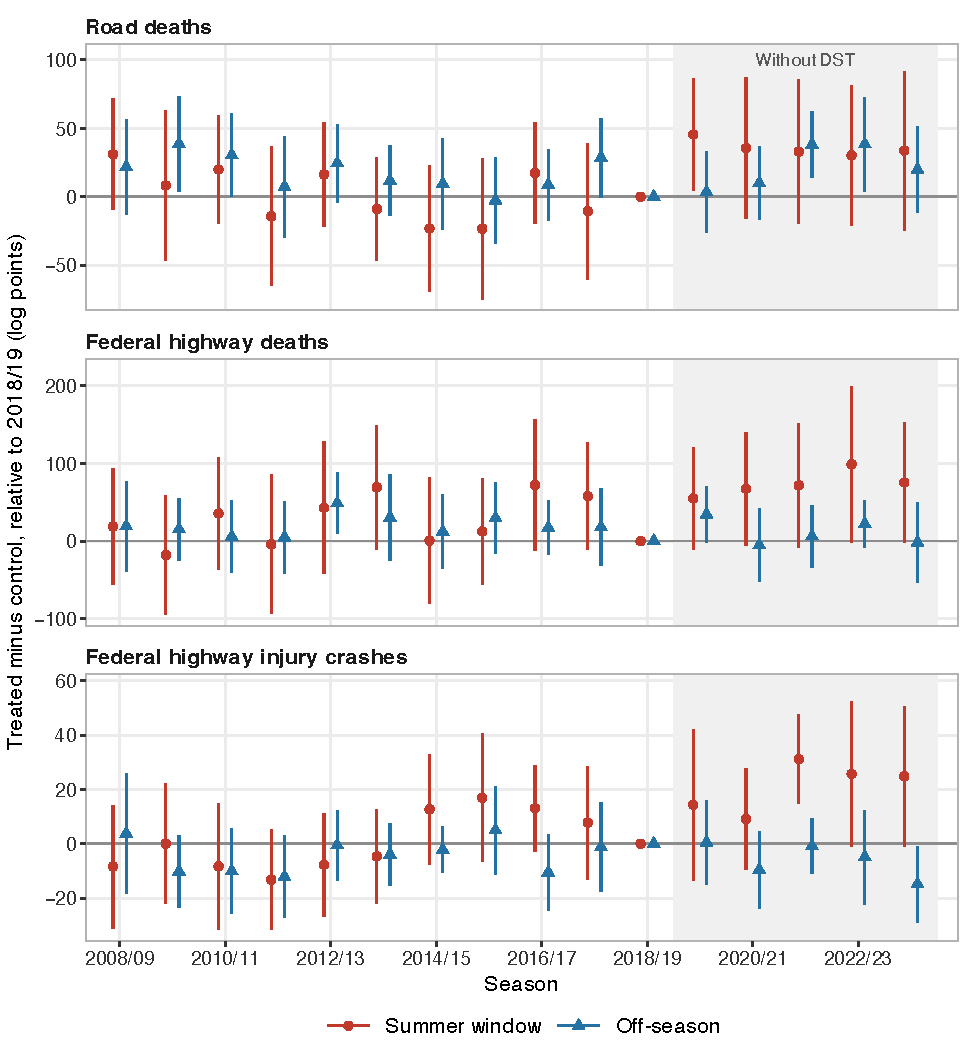
\includegraphics{fig_window_legs.pdf}
  \caption{The Two Legs of the Triple Difference, Season by Season}
  \label{fig:window-legs}
  \begin{figurenotes}[Notes]
  Hour after standard-time sunset. Each point is the coefficient on the treated states in one season from a Poisson model of the summer window alone or of the off-season alone, with state and date effects, against 2018/19. Up to its common date effects, the triple difference is the summer coefficient minus the off-season coefficient; Figure~\ref{fig:event-study} shows it against the average season with DST rather than 2018/19. 95 percent confidence intervals, standard errors clustered by state.
  \end{figurenotes}
  \begin{figurenotes}[Sources]
  \citet{datasus2025sim}; \citet{prf2025dados}.
  \end{figurenotes}
\end{figure}

Figure~\ref{fig:window-legs} shows where the season-to-season swings of the triple difference come from. In the summer window, the gap between treated and control states in hour 0 rose with abolition and stayed at about the same level in all five seasons without DST. In the off-season, which has no change of light, the gap was low in 2019/20, whose off-season includes April to June 2020, and high in 2021/22 and 2022/23. The larger triple-difference estimates of the first two seasons therefore come from the off-season leg. In the summer window alone, the first two summers give 39.3 (12.4) and the last three 31.2 (15.8). Without any day from March 2020 to February 2022, the triple difference gives 36.9 (19.4) for 2019/20 and 18.7 (11.3) for the last two summers.

\subsection{State-by-day fixed effects and sensitivity to trends}

\begin{figure}[tbp]
  \centering
  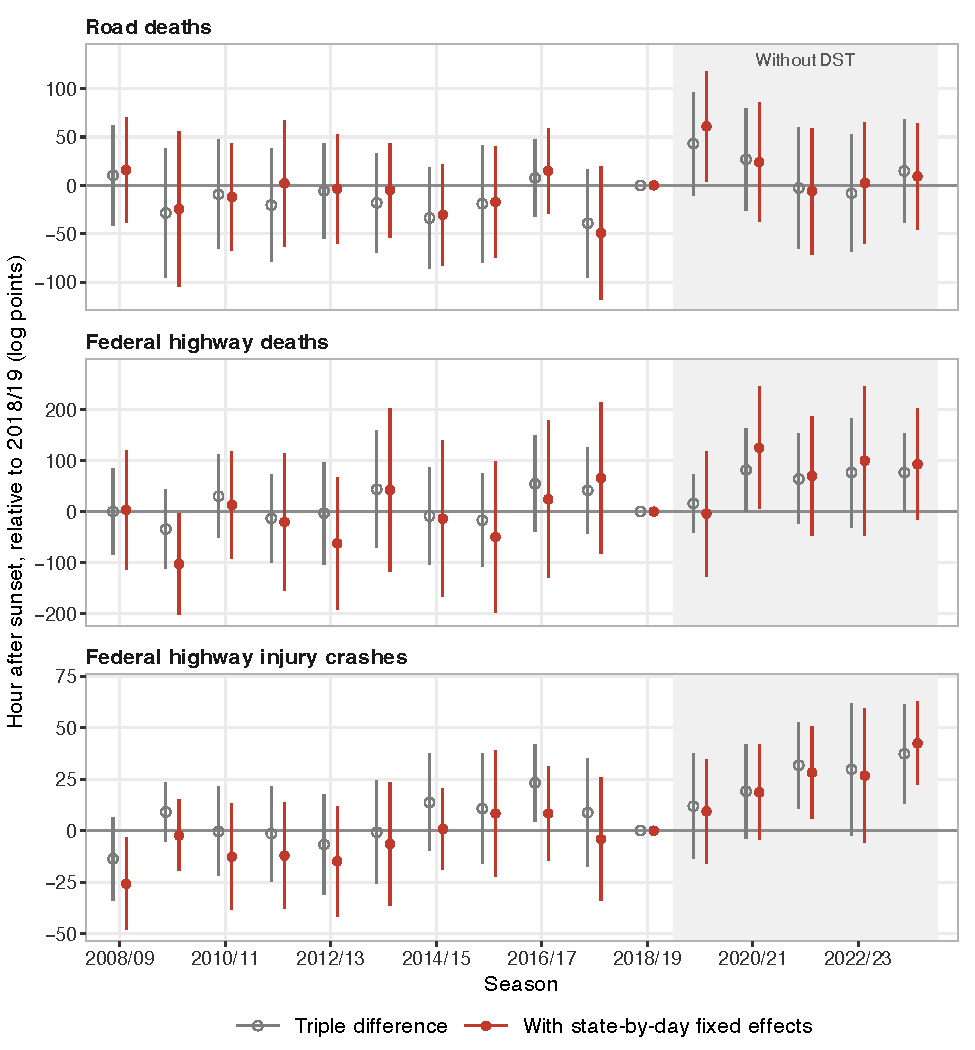
\includegraphics{fig_within_day.pdf}
  \caption{The Hour after Sunset with State-by-Day Fixed Effects}
  \label{fig:within-day}
  \begin{figurenotes}[Notes]
  Grey: hour 0 in Figure~\ref{fig:event-study}. Red: the same hour estimated against hours 3 to 5 before and 2 to 4 after sunset of the same state and day, with state-by-day fixed effects and the fixed effects of equation~(\ref{eq:main}) interacted with the hour. Both against the average of the seasons with DST, as in Figure~\ref{fig:event-study}. 95 percent confidence intervals, standard errors clustered by state.
  \end{figurenotes}
  \begin{figurenotes}[Sources]
  \citet{datasus2025sim}; \citet{prf2025dados}.
  \end{figurenotes}
\end{figure}

Figure~\ref{fig:within-day} repeats the event study with a fixed effect for every state and day, which absorbs any shock common to all hours of a state's day, such as rain, a holiday or the volume of traffic. Pooled over the seasons after abolition, the estimate for road deaths is 27.7 log points (12.4; Table~\ref{tab:robustness}); the standard error does not fall, because the noise in a single hour's count is sampling noise rather than daily shocks.

\begin{table}[tbp]
  \caption{Within the Day, Treated and Control States Each Alone}
  \label{tab:within-group}
  \centering\footnotesize
  \input{\tabdir/tab_within_group.tex}
  \begin{tablenotes}[Notes]
  Hour 0 against hours of the same state and day whose light did not change (evening: 3 to 5 hours before and 2 to 4 after standard-time sunset; morning: 2 to 4 hours before and after standard-time sunrise), summer window against off-season, after abolition against before, estimated in each group separately with state-by-day effects and the fixed effects of equation~(\ref{eq:main}) interacted with the hour; the hours in between, whose light changed in part, have their own coefficients. Column 4: vehicles at federal highway count stations, with station-by-day and station-by-hour effects. Standard errors clustered by state.
  \end{tablenotes}
  \begin{tablenotes}[Sources]
  \citet{datasus2025sim}; \citet{prf2025dados}; \citet{dnit2025pnct}.
  \end{tablenotes}
\end{table}

The control states kept their clocks, but schedules set on Bras\'ilia time, such as national broadcasts, ran an hour earlier on those clocks in every summer with DST and have run at the same clock time all year since. If that change moved the control states' evening, they would not supply the counterfactual the triple difference assumes. Table~\ref{tab:within-group} compares hour 0 with hours of the same state and day whose light did not change, in each group alone. Traffic did not move in the control states' evening: vehicles in hour 0 changed by $-0.2$ log points (0.7), against $-5.4$ (1.6) in the treated states. Road deaths in the control states' hour 0 did rise relative to the rest of their day, by 19.7 log points (6.5), while their federal highway deaths and injury crashes in that hour fell. Whatever raised those deaths did not move traffic. To the extent that it came from the control states' own schedules, the triple difference understates the effect: within the treated states alone, road deaths in hour 0 rose by 47.2 log points (7.8). In the morning, road deaths in hour 0 fell in both groups and traffic rose in both, so the triple difference nets out a change the control states share. Within the treated states alone, road deaths in the morning hour that turned light fell by 19.4 log points (9.6). Applied to the 107 and 110 deaths per summer the two hours had before abolition, that fall offsets less than a third of the evening rise.

\begin{figure}[tbp]
  \centering
  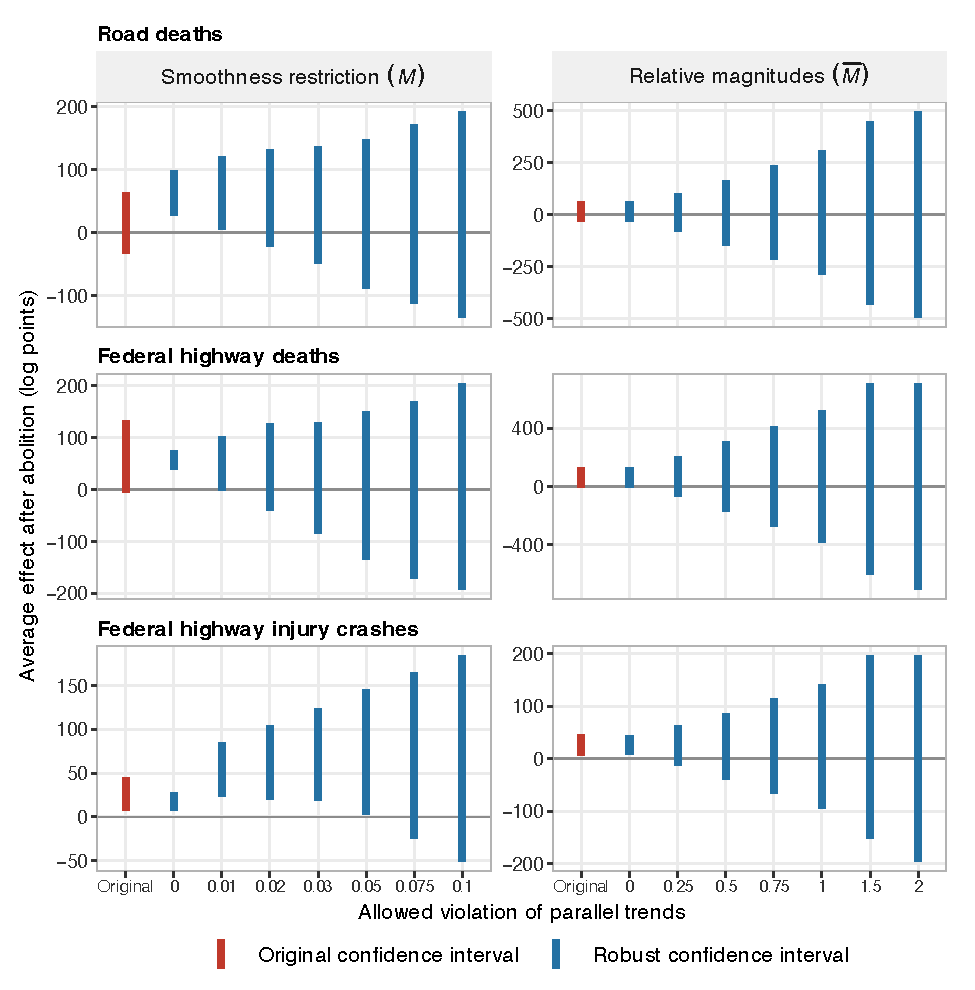
\includegraphics{fig_honestdid.pdf}
  \caption{Sensitivity to Violations of Parallel Trends}
  \label{fig:honestdid}
  \begin{figurenotes}[Notes]
  95 percent confidence intervals for the average of the five season coefficients after abolition in Figure~\ref{fig:event-study}, hour 0 \citep{rambachan2023more}. These coefficients are measured against 2018/19, not against the average of the seasons before abolition, so the target differs from $\beta$ in Table~\ref{tab:main}. Left: the slope of the violation may change by at most $M$ between seasons, in log units (0.01 is 1 log point). Right: the violation after abolition is at most $\bar M$ times the largest one before it.
  \end{figurenotes}
  \begin{figurenotes}[Sources]
  \citet{datasus2025sim}; \citet{prf2025dados}.
  \end{figurenotes}
\end{figure}

Figure~\ref{fig:honestdid} reports the sensitivity analysis of \citet{rambachan2023more} for the average post-abolition coefficient of the event study. The method measures the violations of parallel trends from a single reference season, so here the coefficients are taken against 2018/19, not against the average season with DST as in Figure~\ref{fig:event-study}. For road deaths that average is 14.8 log points, and its conventional interval already includes zero, because a single reference season is a noisy baseline. If the pre-abolition trend is extended linearly ($M=0$), the interval is 28 to 99 log points; allowing its slope to change by 0.02 per season (2 log points) brings zero into it. % honestdid.rds.
The event study therefore cannot rule out departures from parallel trends of the size of its own season-to-season noise, which is why the paper's case rests on the pattern within the day.

\subsection{Who dies}

\begin{table}[tbp]
  \caption{Who Dies in the Hour That Turned Dark}
  \label{tab:road-users}
  \centering\footnotesize\setlength{\tabcolsep}{5pt}
  \input{\tabdir/tab_road_users.tex}
  \begin{tablenotes}[Notes]
  Road deaths in hour 0, equation~(\ref{eq:main}) estimated separately for each group, standard errors clustered by state. Road users from the ICD-10 block of the underlying cause (Appendix~\ref{app:data}); 85 percent of the other road users who died in hour 0 have no vehicle specified (V87 to V89), 10 percent were in heavy transport vehicles and the rest in buses, three-wheeled or other vehicles. Weekends and holidays: Saturdays, Sundays and national holidays (fixed dates, Carnival Monday and Tuesday, Good Friday); the last row of Panel C also drops the Saturday before Carnival to Ash Wednesday and 24 December to 1 January. Dashes: fewer than five deaths per summer in the treated states before abolition, too few to estimate.
  \end{tablenotes}
  \begin{tablenotes}[Source]
  \citet{datasus2025sim}.
  \end{tablenotes}
\end{table}

Table~\ref{tab:road-users} splits road deaths in hour 0 by road user, by the age and sex of pedestrians, and by type of day. Among pedestrians, deaths of those aged 15 to 64, two thirds of the total, rose by 91.1 log points (30.9); the other age groups are too small to estimate. Motorcyclists rise by 19.6 (10.9); the estimate for car occupants is close to zero and imprecise ($-0.2$, 35.2); the residual group, mostly deaths with no type of vehicle recorded, rises by 55.8 (26.4). The estimate on weekends and holidays (41.3, 15.8) is larger than on working days (16.1, 10.0), and stays so without Carnival and the year-end holidays (39.3, 16.2).

\begin{table}[tbp]
  \caption{Sex and Age of the Dead in the Hour That Turned Dark}
  \label{tab:sex-age}
  \centering\footnotesize\setlength{\tabcolsep}{3pt}
  \input{\tabdir/tab_sex_age.tex}
  \begin{tablenotes}[Notes]
  Equation~(\ref{eq:main}) for hour 0, estimated separately for the dead of each sex and age group, standard errors clustered by state. Road deaths: sex and age from the death certificate. Federal highway deaths: sex and age from the police record of each person in the crash; the age of 12 percent of the dead is not recorded before 2017 and of 6 percent from 2017, when the record began to enter a missing age as zero, which is treated as not recorded. Deaths per summer: mean in the treated states' summer window before abolition. Dashes: fewer than five deaths per summer, too few to estimate.
  \end{tablenotes}
  \begin{tablenotes}[Sources]
  \citet{datasus2025sim}; \citet{prf2025dados, prf2025pessoas}.
  \end{tablenotes}
\end{table}

Table~\ref{tab:sex-age} splits the dead in hour 0 by sex and age in both registers. Men are about four fifths of the dead in both. Their road deaths rose by 33.8 log points (9.9) and their federal highway deaths by 65.2 (20.7); the estimates for women, 12.7 (22.2) and 5.8 (42.3), are too imprecise to say whether their deaths rose less. Every age group from 15 years on has a positive estimate in road deaths, and so does every group on federal highways with enough deaths to estimate. Their intervals overlap too much to rank them.

\subsection{Traffic volume and risk per vehicle}

\begin{table}[tbp]
  \caption{Traffic Volume and Risk per Vehicle on Federal Highways}
  \label{tab:volume}
  \centering\footnotesize
  \input{\tabdir/tab_traffic_volume.tex}
  \begin{tablenotes}[Notes]
  Log points, standard errors clustered by state in parentheses, permutation p-values in brackets. Column 1: equation~(\ref{eq:main}) on hourly vehicle counts at continuous counting stations, with station fixed effects; summers 2014/15 to 2018/19 and 2021/22 to 2024/25. Column 2: the 30 pairs formed by a station counted only after abolition within 2 km of one counted only before on the same highway, with pair-by-window and pair-by-season effects in place of the state effects. Columns 3 and 5: as in Table~\ref{tab:main}, on the same summers as column 1. Per vehicle: crash or death estimate minus the volume estimate of column 1. Every column is re-estimated with the same random set of 11 treated states in each of 999 draws, so the per-vehicle columns have their own reference distribution; permutation tests are on t-statistics, a per-vehicle difference divided by the square root of the sum of its two squared standard errors.
  \end{tablenotes}
  \begin{tablenotes}[Sources]
  \citet{dnit2025pnct}; \citet{prf2025dados}.
  \end{tablenotes}
\end{table}

Table~\ref{tab:volume} reports, for the seven hours around sunset and sunrise, the triple difference on hourly vehicle counts at federal highway stations (column 1), on federal highway injury crashes and deaths (columns 3 and 5), and their difference, the change per vehicle (columns 4 and 6). Because no station is counted both before and after abolition, the volume model has station fixed effects and the seasonal comparison runs at the level of the state, as in equation~(\ref{eq:main}). Column 2 follows the 30 stations that were moved at most 2 kilometers along the same highway, as pairs: the evening falls are smaller there and the morning rise larger. The crash columns come from the same summers as the volume, on which hour 0 shows no pre-abolition trend in injury crashes. Section~\ref{sec:traffic} of the paper discusses hour 0, the hour before sunset and the hour after sunrise.

\subsection{Rain and street lighting}

On a rainy, overcast evening the hour was already dim under DST, so abolition should darken it less. Panel B of Table~\ref{tab:sensitivity} points that way for every outcome, without precision: for road deaths, the effect on a dry state-day is 43.5 log points (15.5) and the change from a dry to a fully rainy state-day $-4.3$ (34.4). Controlling for the share of the state under rain leaves the main estimate at 29.1.

\begin{table}[tbp]
  \caption{Street Lighting}
  \label{tab:lighting}
  \centering\footnotesize
  \input{\tabdir/tab_street_lighting.tex}
  \begin{tablenotes}[Notes]
  Municipalities split within each state at the median, weighted by road deaths before abolition, of the share of households on a street face without public lighting: Census 2022 in Panels A and B, urban tracts of Census 2010 in Panel C. The municipality that crosses the median goes to the darker half; the Federal District, a single municipality, falls wholly in it. Equation~(\ref{eq:main}) on the panel of states by half by day, with every fixed effect interacted with the half; standard errors clustered by state.
  \end{tablenotes}
  \begin{tablenotes}[Sources]
  \citet{ibge2023censo}; \citet{ibge2011censo}.
  \end{tablenotes}
\end{table}

If darkness kills pedestrians, street lighting should blunt the effect. Table~\ref{tab:lighting} splits the municipalities of each state into a darker and a better-lit half by the share of households on streets without public lighting. With the 2022 Census, the estimate for road deaths is 42.5 log points (10.0) in the darker half and 10.9 (16.0) in the better-lit half; the difference has the predicted sign but $p=0.10$. With the 2010 Census the gap is smaller (37.1 against 22.9). The halves also differ in the hour before sunset, whose light changed only in degree (Panel B), so the split may capture other differences between municipalities. We read the table as consistent with a role for street lighting, not as evidence of one.

\subsection{Valuing the deaths}\label{app:cost}

Table~\ref{tab:cost} scales the net count of the darkness dose model (Table~\ref{tab:excess}, Panel A) with two ratios, both from land-transport deaths in the treated states' summer window before abolition. The whole-season count adds, for each season after abolition, the days of the 2017 rule's DST season outside the summer window: the first Sunday of November to 14 November and 15 February to the day before the third Sunday of February (a week later when that Sunday was Carnival), 15.8 days a season on average. Their excess deaths apply the dose coefficients of the summer window to the deaths observed on those days. Column 2 multiplies column 1 by the ratio of road deaths per summer to those with a valid clock time, $2{,}933/2{,}382 = 1.231$. Column 3 multiplies column 2 by the ratio of all land-transport deaths to road deaths, $6{,}003/2{,}933 = 2.047$. Of the land-transport deaths off the road, 84.9 percent occurred in hospital, 9.7 percent at another place, 3.5 percent in another health facility, 1.5 percent at home and 0.4 percent at an unknown place. % total_cost.rds, scale; SIM LOCOCOR, treated summer window, 2008/09-2018/19.

The value of a statistical life follows the three rules of \citet{robinson2019valuing}, with $Y$ the gross national income per head at purchasing power parity in 2025, $Y_{\mathit{BR}} = 22{,}670$ and $Y_{\mathit{US}} = 89{,}490$ international dollars \citep{worldbank2026wdi}:
\begin{align*}
  \text{(a)}\quad \mathit{VSL} &= \max\{160\, Y_{\mathit{US}}\, (Y_{\mathit{BR}}/Y_{\mathit{US}})^{1.5},\; 20\, Y_{\mathit{BR}}\} = 1{,}825{,}618, \\
  \text{(b)}\quad \mathit{VSL} &= 160\, Y_{\mathit{BR}} = 3{,}627{,}200, \\
  \text{(c)}\quad \mathit{VSL} &= 100\, Y_{\mathit{BR}} = 2{,}267{,}000.
\end{align*}
Rule (a) is the default of \citet{robinson2019valuing}: it starts from the US ratio of VSL to income per head and lets the ratio fall with income, down to a floor of 20 times income per head, which does not bind here (453,400). Rule (b) applies the US ratio and rule (c) the OECD ratio directly to Brazilian income. The values are in 2025 international dollars, the unit of $Y$, and Table~\ref{tab:cost} reports the value of the deaths in that unit. At the 2025 purchasing-power-parity conversion factor for GDP, 2.554 reais per international dollar \citep{worldbank2026wdi}, they are R\$4.66, 9.27 and 5.79 million.

The human-capital alternative is the cost per person killed in a fatal crash on a federal highway, R\$433,287 in December 2014 prices, almost all of it lost production \citep[Table 6A]{ipea2015acidentes}. Multiplied by the ratio of the IPCA consumer price index in December 2025 to December 2014, $7{,}403.29/4{,}059.86 = 1.824$ \citep{ibge2026ipca}, it is R\$790,113, or 309,313 international dollars at the same conversion factor. Each value in Table~\ref{tab:cost} is the count of deaths times the value of one death; the standard errors treat the scaling ratios and the values as fixed.

\subsection{The clock changes before abolition}

\begin{table}[tbp]
  \caption{The Clock Changes before 2019 and Abolition}
  \label{tab:transitions}
  \centering\footnotesize
  \input{\tabdir/tab_transitions.tex}
  \begin{tablenotes}[Notes]
  Abolition: Table~\ref{tab:main} (Panel A) and the state-by-day row of Table~\ref{tab:robustness} (Panel B). Clock changes: days within 21 days of each change of the seasons 2008/09 to 2018/19, at the dates of the decrees, and the same calendar days of the seasons 2019/20 to 2023/24 at the dates the 2008 rule would have set (third Sunday of October; third Sunday of February, a week later on Carnival Sunday), when no clock moved. Panel A: $y_{sd} = \exp(\beta\, T_s \times \textit{after}_d \times \textit{DST era}_d + \text{state} \times \text{season} + \text{state} \times \textit{after} + \text{date})$. Panel B: hour 0 against hours 3 to 5 before and 2 to 4 after sunset of the same state and day, with state-by-day effects and the other effects interacted with the hour. The average of the two is the February estimate minus the October estimate, divided by two: reversing the sign of the October change reads both as the effect of a darker evening. Both changes enter one model with every effect interacted with the change, so the average has a clustered standard error. The difference from abolition comes from a model that also stacks the abolition panel, every fixed effect interacted with the experiment and standard errors clustered by state across all three, so the overlap of the samples (the weeks before the February change fall in the summer window) enters its standard error; each coefficient equals its separate estimate. The school-week rows split the abolition effect into the school weeks of the summer window (15 November to 7 December), the school holidays (24 December to 15 January) and the other days, as in Table~\ref{tab:sensitivity}, and stack it with the two changes in the same way.
  \end{tablenotes}
  \begin{tablenotes}[Sources]
  \citet{datasus2025sim}; \citet{prf2025dados}.
  \end{tablenotes}
\end{table}

Table~\ref{tab:transitions} reports the comparison of Section~\ref{sec:transitions}. The seasons after abolition enter only to net out the change in deaths from the weeks before to the weeks after mid-October and mid-February that has nothing to do with the clock. Panel B is the cleaner comparison for the clock changes, because each change also moves an hour of sleep, lost in October and gained in February, and that acts on every hour of the day: an October rise from lost sleep and a February fall from gained sleep would both push the hour-0 estimates of Panel A toward zero. The clock changes give larger point estimates for road deaths than abolition in both panels, but the difference is distinguishable from zero only in Panel B ($-51.4$, standard error 18.3); in Panel A it is $-13.1$ (12.5). The changes fall in term time, and most of the summer window does not. Against abolition in the school weeks of the window, the difference is 15.8 (18.0) in Panel A and $-22.2$ (20.9) in Panel B, so in the same part of the school year the two settings cannot be told apart. For federal highway deaths it is distinguishable only in Panel A, and federal highway injury crashes give about the same estimate in both settings.

\subsection{Bahia, the one season it had DST}

\begin{figure}[tbp]
  \centering
  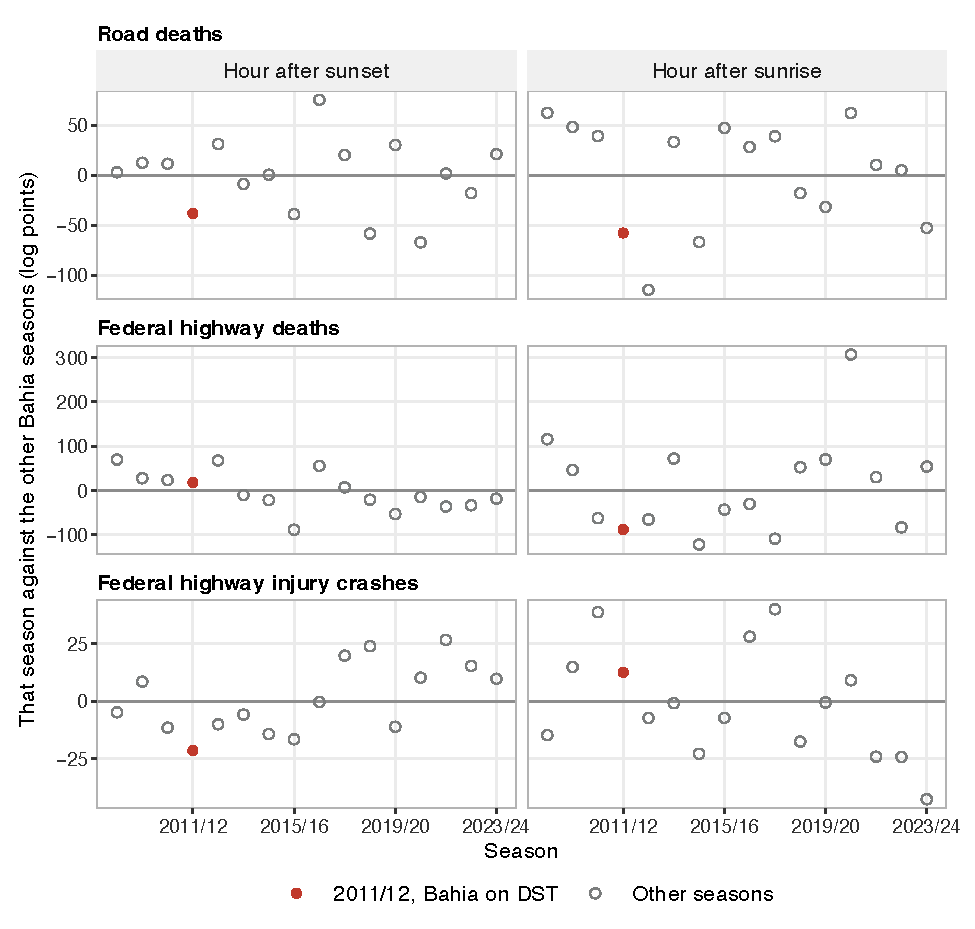
\includegraphics{fig_bahia.pdf}
  \caption{Bahia, the One Season It Had Daylight Saving Time}
  \label{fig:bahia}
  \begin{figurenotes}[Notes]
  Bahia had DST in 2011/12 only. Each point compares one Bahia season with all its other seasons, against the control states, summer window against off-season, in the hour after standard-time sunset (left) or sunrise (right). The main result predicts the 2011/12 point to be the lowest on the left and the highest on the right.
  \end{figurenotes}
  \begin{figurenotes}[Sources]
  \citet{datasus2025sim}; \citet{prf2025dados}.
  \end{figurenotes}
\end{figure}

Bahia, excluded from the main sample, had DST in a single summer, 2011/12. That summer its hour 0 was light, and in every other summer it was dark, so the main result predicts that Bahia's hour 0 had unusually few events in 2011/12. The first stage is clear: officers recorded 68 percent of Bahia's crashes in hour 0 as dusk or night in 2011/12, against 93 to 100 percent in every other season. % bahia_switch.rds, first_stage.
Tocantins, which had DST only in 2012/13, is too small for the same check: its hour 0 had about 9 federal highway injury crashes and 2 federal highway deaths per summer, against 57 and 13 in Bahia, so a single season's estimate could not be distinguished from noise. % PRF injury crashes and deaths in evening hour 0, summer window, 2008/09-2023/24: TO 8.8 and 2.0, BA 57.1 and 13.2 per season.
Figure~\ref{fig:bahia} ranks the 2011/12 estimate among Bahia's 16 seasons for each outcome. In the evening, federal highway injury crashes are the lowest of the 16 ($-21.4$ log points), road deaths the fourth lowest and federal highway deaths the eleventh lowest. In the morning the prediction fails: road deaths and federal highway deaths in 2011/12 rank third lowest, and injury crashes twelfth lowest. With one state and one season, the lowest rank of 16 corresponds to a one-sided p-value of about 0.06. We show all six comparisons as a check of sign, not as an estimate.

\subsection{Assault deaths}

\begin{figure}[tbp]
  \centering
  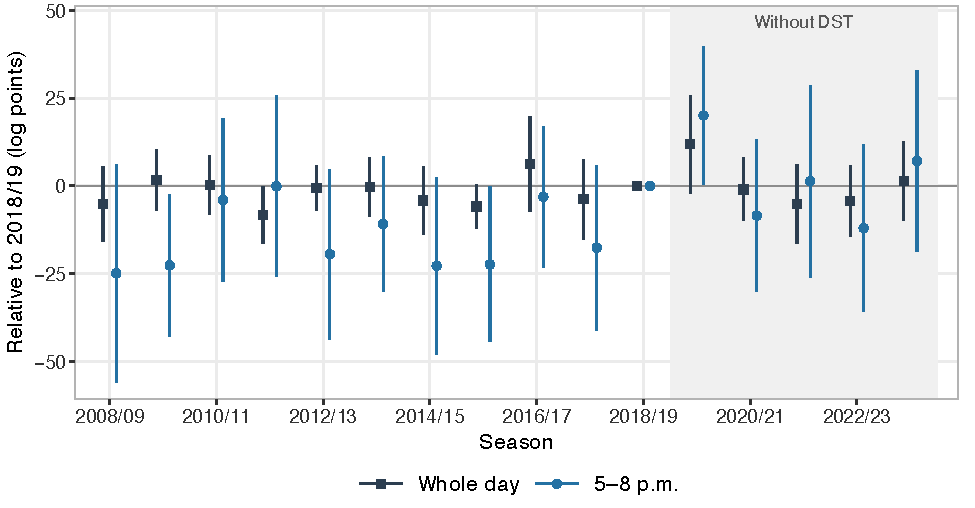
\includegraphics{fig_assault.pdf}
  \caption{Assault Deaths, Season by Season}
  \label{fig:assault}
  \begin{figurenotes}[Notes]
  Deaths from assault (ICD-10 X85--Y09) in any place, by clock time of death. Equation~(\ref{eq:main}) by season as in Figure~\ref{fig:event-study}, for the whole day and for 5 to 8 p.m.\ clock time. 95 percent confidence intervals, standard errors clustered by state.
  \end{figurenotes}
  \begin{figurenotes}[Source]
  \citet{datasus2025sim}.
  \end{figurenotes}
\end{figure}

Ambient light also affects crime \citep{doleac2015under, dominguez2023crime}, so we examined deaths from assault with the same design. They show no signature of light (Figure~\ref{fig:assault}). The whole-day triple difference is 2.4 log points (1.7), and $-0.5$ (1.5) without 2019/20, the one season in which the coefficients jump. Between 8 a.m.\ and 5 p.m., hours whose light did not change, the estimate (7.0, 2.6) is of the same order as between 5 and 8 p.m.\ (15.2, 5.0). % assault_trends.rds, results.
A change in violence concentrated in one season and spread across the day is not an effect of light, and the paper does not study assault deaths further. The triple difference can thus find changes after 2019 in hours whose light did not change; for road deaths, Panel D of Table~\ref{tab:robustness} finds none.


\end{document}
